\documentclass{article}
\usepackage[utf8]{inputenc}
\usepackage[english]{babel}
\usepackage{enumitem}
\usepackage{amsthm}
\newtheorem{theorem}{Theorem}
\newtheorem{proposition}{Proposition}
\newtheorem{definition}{Definition}
\usepackage{float}
\usepackage{lineno,hyperref}
\modulolinenumbers[5]
\usepackage{amssymb}
\usepackage{amsmath}
\usepackage{url}
\usepackage{multirow}
\usepackage{graphicx}
\graphicspath{{./figures/}{./}}
\usepackage{fancyhdr}
\usepackage{hyperref}
\usepackage{xcolor}
\usepackage{tikz}
\usepackage{pgfgantt}
\usepackage{listings}
\usepackage{courier}

\lstset{
    basicstyle=\ttfamily\small,
    breaklines=true,
    numbers=left,
    numberstyle=\tiny,
    keywordstyle=\color{blue},
    commentstyle=\color{gray},
    stringstyle=\color{red},
}
\lstdefinestyle{codeblock}{
    backgroundcolor=\color{gray!10},
    basicstyle=\ttfamily\small,
    breaklines=true,
    frame=single,
    rulecolor=\color{black!50},
    numbers=left,
    numberstyle=\tiny\color{gray},
    numbersep=12pt,
    xleftmargin=20pt,
    framexleftmargin=20pt,
    framextopmargin=5pt,
    framexbottommargin=5pt,
    keywordstyle=\color{blue},
    stringstyle=\color{red!70!black},
    commentstyle=\color{green!50!black},
    tabsize=2
}

\usepackage[margin=2.5cm]{geometry}

\usepackage{booktabs}
\usepackage{amssymb}
\usepackage{multirow}
\usepackage{array}
\usepackage{makecell}
\newcolumntype{L}[1]{>{\raggedright\let\newline\\\arraybackslash\hspace{0pt}}m{#1}}
\newcolumntype{C}[1]{>{\centering\let\newline\\\arraybackslash\hspace{0pt}}m{#1}}
\newcolumntype{R}[1]{>{\raggedleft\let\newline\\\arraybackslash\hspace{0pt}}m{#1}}

\usepackage{mathtools}
\usepackage{setspace}

\definecolor{barblue}{RGB}{153,204,254}
\definecolor{groupblue}{RGB}{51,102,254}
\definecolor{linkred}{RGB}{165,0,33}
\definecolor{phgray}{RGB}{200,200,200}
\definecolor{phbg}{RGB}{245,245,245}

% ----------------------------------------------------------------------------
% Screenshot placeholder. Use this in place of \includegraphics for figures
% the user will fill in later. Replace \screenshotplaceholder{<filename>}{<label>}
% with \includegraphics[width=0.95\linewidth]{<filename>} once the screenshot
% has been dropped into the figures/ folder.
% ----------------------------------------------------------------------------
\newcommand{\screenshotplaceholder}[2]{%
  \begin{tikzpicture}
    \draw[fill=phbg, draw=phgray, thick, dashed]
      (0,0) rectangle (\linewidth - 0.4pt, 7cm);
    \node[align=center, text=gray] at (0.5\linewidth, 4cm)
      {\textsc{\large Screenshot placeholder}};
    \node[align=center, text=gray] at (0.5\linewidth, 3.2cm)
      {Drop \texttt{#1} into \texttt{./figures/} and replace};
    \node[align=center, text=gray] at (0.5\linewidth, 2.6cm)
      {this command with \texttt{\textbackslash includegraphics}};
    \node[align=center, font=\itshape\small, text=gray!80!black]
      at (0.5\linewidth, 1.4cm) {#2};
  \end{tikzpicture}%
}

\title{}
\author{}
\date{}

% ----------------------------------------------------------------------------
% Title page
% ----------------------------------------------------------------------------
\newcommand*{\titleGP}{\begingroup
    \centering
    \vspace*{\baselineskip}

    \rule{\textwidth}{1.6pt}\vspace*{-\baselineskip}\vspace*{2pt}
    \rule{\textwidth}{0.4pt}\\[\baselineskip]
    {\LARGE Quner: Modular AI Framework for Intelligent Healthcare Training Systems} \\

    \rule{\textwidth}{0.4pt}\vspace*{-\baselineskip}\vspace{3.2pt}
    \rule{\textwidth}{1.6pt}\\[\baselineskip]

    \scshape
    \vspace*{1\baselineskip}
    {\large{\textsl{
            \LARGE \bf Project Report for MAJOR PROJECT II
    }}}\\[2ex]
    {\large{\textsl{
            submitted in partial fulfillment of the requirements for the award of the degree of \\[1ex]\textbf{Bachelor of Technology} \\in \\\textit{Computer Science \& Engineering}
    }}}\\[4ex]

    \emph{by} \\[1ex]
    \begin{table}[ht]
        \centering
        \begin{tabular}{|c|c|}
            \hline
            \textbf{Name} & \makecell{\textbf{Enrollment Number}} \\
            \hline \hline
            \makecell{Yash Tamar} & \makecell{R2142221249} \\
            \hline
            \makecell{Milind Vishwakarma} & \makecell{R2142221227} \\
            \hline
        \end{tabular}
    \end{table}
    \emph{} \\[1ex]
    {\normalfont \emph{Under the supervision of}} \\
    [\baselineskip]
    \large {\bf Mr. Mohd Farooq}\\
    {\normalfont Assistant Professor \\
    Department of Computer Science}

    \vfill
    
\includegraphics[scale=0.8]{UPES-Logo-without-Tagline.jpg}\\
    \vfill

    {\scshape February -- May 2026} \\[0.3\baselineskip]
    {School of Computer Science}\\[0.3\baselineskip]
    {\large University Of Petroleum and Energy Studies}\\[0.3\baselineskip]
    {\normalfont Dehradun-248007}\par
    \thispagestyle{empty}

\endgroup}

\begin{document}

\maketitle
\vspace{-2.5cm}
\titleGP
\clearpage

% ----------------------------------------------------------------------------
% Candidate's declaration
% ----------------------------------------------------------------------------
\begin{center}
    \Large \textbf{CANDIDATE'S DECLARATION}
\end{center}

\vspace{1cm}

We hereby certify that the project work entitled \textbf{``Quner: Modular AI Framework for Intelligent Healthcare Training Systems''} in partial fulfillment of the requirements for the award of the Degree of \textbf{BACHELOR OF TECHNOLOGY} in \textbf{COMPUTER SCIENCE AND ENGINEERING} with specialization in \textbf{Data Science, Big Data and Artificial Intelligence and Machine Learning} respectively, submitted to the School of Computer Science, UPES, Dehradun, is an authentic record of our work carried out during a period from \textbf{February, 2026} to \textbf{May, 2026} under the supervision of \textbf{Mr. Mohd Farooq, Assistant Professor, Department of Computer Science}.

\vspace{1cm}

The matter presented in this project has not been submitted by us for the award of any other degree of this or any other University.

\vspace{1.5cm}

\begin{center}
    \begin{tabular}{|c|c|}
        \hline
        \textbf{Name} & \textbf{Enrollment Number} \\
        \hline \hline
        Yash Tamar & R2142221249 \\
        \hline
        Milind Vishwakarma & R2142221227 \\
        \hline
    \end{tabular}
\end{center}

\vspace{1.5cm}

This is to certify that the above statement made by the candidate is correct to the best of my knowledge.

\vspace{3cm}

\noindent
Date: \underline{\hspace{3cm}} 2026
\hfill
\begin{minipage}{6cm}
    \centering
    \textbf{Mr. Mohd Farooq}\\
    Project Guide
    \vspace{1.5cm}
\end{minipage}

\vspace{5cm}
\hrule
\newpage

% ----------------------------------------------------------------------------
% Acknowledgement
% ----------------------------------------------------------------------------
\begin{center}
    \Large \textbf{Acknowledgement}
\end{center}

We wish to express our deep gratitude to our guide \textbf{Mr. Mohd Farooq}, for all the advice, encouragement and constant support he has given us throughout our project work. This work would not have been possible without his support and valuable suggestions. We sincerely thank our respected \textbf{Dr. Virender Kadyan}, Head, Department of \underline{\textbf{Data Science}}, for his great support in doing our project on \underline{\textbf{Quner: Modular AI Framework for Intelligent Healthcare Training Systems}}. We are also grateful to the Dean, SoCS UPES, for giving us the necessary facilities to carry out our project work successfully. We also thank our Course Coordinator, \textbf{Dr. Neeraj Chugh}, and our Activity Coordinator, \textbf{Dr. Khushboo Jain}, for providing timely support and information during the completion of this project. We would like to thank all our friends for their help and constructive criticism during our project work. Finally, we express our sincere gratitude to our parents who have shown us this world and for every support they have given us.

\vspace{1cm}

\begin{center}
    \begin{tabular}{|c|c|}
        \hline
        \textbf{Name} & \textbf{Enrollment Number} \\
        \hline \hline
        Yash Tamar & R2142221249 \\
        \hline
        Milind Vishwakarma & R2142221227 \\
        \hline
    \end{tabular}
\end{center}

\newpage

% ----------------------------------------------------------------------------
% Contents
% ----------------------------------------------------------------------------
\lhead{\emph{Contents}}
\tableofcontents
\thispagestyle{empty}
\cleardoublepage
\typeout{}

\setstretch{1.2}
\pagenumbering{arabic}

\begin{center}
    \huge \textbf{Quner}
\end{center}

% ----------------------------------------------------------------------------
% Abstract
% ----------------------------------------------------------------------------
\section{Abstract}
This project presents \textbf{Quner}, a modular agentic-AI framework that automates the full clinical-skills training cycle for medical students. The system orchestrates three cooperating agents -- a \emph{Generator agent} that produces evidence-based-medicine grounded vignettes with configurable Big-Five personalities, a \emph{Virtual Simulated Patient (VSP) agent} that holds persona-consistent clinical interviews, and a \emph{Critic agent} that delivers MIRS-aligned communication feedback alongside structured clinical evaluation \cite{Kulkarni2023TheEO,Topsakal2023CreatingLL}. Conversation flows through a single asynchronous WebSocket hub that decouples the agents from the user-facing dashboard, allowing the same backend to drive a browser chat client, a Furhat robotic head, or both \cite{Plale2013BigDO}. A pluggable \emph{pipeline mode} lets the same code route through OpenAI, Groq's free tier, or the original Cerebras + Groq + OpenAI mix, while a Pinecone-backed RAG layer can be turned on for clinical grounding when desired \cite{Monir2024VectorSearchED}. The browser dashboard supports text chat, push-to-talk speech input via the Web Speech API with optional auto-submit, system-default text-to-speech for patient replies, an on-demand "Hint" button that asks the Critic agent for a one-sentence next-step suggestion, and a slide-out vignette drawer for quick reference \cite{Zhang2023SentimentAI}. Compared to traditional standardized-patient programmes, Quner reduces the marginal cost of one practice session to fractions of a cent while still producing structured, rubric-aligned feedback aligned with the Master Interview Rating Scale (MIRS) \cite{Jing2024WhenLL}.

% ----------------------------------------------------------------------------
% Introduction
% ----------------------------------------------------------------------------
\section{Introduction}

Medical education depends heavily on \emph{simulated practice}: students need a safe space to develop clinical interviewing, history-taking, and reasoning skills before they meet real patients. Traditional simulation programmes rely on standardized-patient (SP) actors, dedicated faculty time, and physical simulation suites \cite{Portovaras2024CurrentTA}. These resources are scarce, expensive, and difficult to scale: a typical Objective Structured Clinical Examination (OSCE) station occupies a faculty member, an SP actor, and a physical room for the entire window in which a single student is being assessed \cite{Azzara2023PeranPP}.

The recent generation of large language models (LLMs) creates a credible alternative: an LLM-driven \emph{virtual simulated patient} can sustain a fluent multi-turn dialogue, take on a personality, and stay consistent with a clinical vignette for the duration of a session \cite{Topsakal2023CreatingLL}. Existing LLM-driven SPs, however, suffer from three repeatable failure modes \cite{Plale2013BigDO}: (a) \emph{medical inaccuracy}, where the model fabricates symptoms or guidelines that aren't in the case; (b) \emph{persona drift}, where the model breaks character or starts speaking like a doctor; and (c) \emph{evaluative weakness}, where students get a transcript but no structured pedagogical feedback against a recognised rubric.

\textbf{Quner} addresses these failure modes with an explicit \emph{multi-agent architecture}. Each of the three core capabilities -- scenario generation, in-character dialogue, and standards-based feedback -- is owned by a separate agent with its own prompt structure, model selection, and guardrails. The agents communicate through a single WebSocket message bus that also exposes the conversation to one or more user-facing clients. This separation lets each agent be tuned, evaluated, and replaced independently, and it makes the system robust to changes in any one upstream provider \cite{Cheptsov2013IntroducingAN}.

The project began with a research prototype that hard-coded a single set of API keys, was tightly coupled to a Furhat robotic head for I/O, and consisted of a small number of monolithic Python modules. Major Project II takes that prototype and turns it into a deployable, modular system: secrets are externalised, the codebase is split into focused agent and LLM packages, and the dashboard is upgraded with browser-native speech, an on-demand coaching button, and a redesigned single-screen layout \cite{Ren2024AdvancementsAA}.

\subsection{Problem Statement}

Clinical interviewing is taught by \emph{practice}, not by lectures. Yet practice in medical schools is bottlenecked by three tightly coupled scarce resources \cite{Portovaras2024CurrentTA}:
\begin{itemize}
    \item \textbf{Standardized patient actors} who must be recruited, trained, and paid for every cohort and every disease they need to portray.
    \item \textbf{Faculty observers} who score each encounter against the Master Interview Rating Scale (MIRS) or a similar communication rubric.
    \item \textbf{Physical OSCE rooms} which are limited in number and conflict with assessments and other clinical training.
\end{itemize}

The result is that students get a \emph{small number of high-stakes practice sessions}, often clustered around exam season, with low formative feedback density \cite{Plale2013BigDO}. Existing software simulators try to fill the gap, but the current generation of "AI patient" tools share a recurring set of weaknesses \cite{Azzara2023PeranPP}:

\begin{itemize}
    \item Vignettes are static, hand-authored, and shared between students, which limits replay value and exposes test items.
    \item Patient dialogue is driven by a single un-grounded LLM call, which produces fluent text but frequently hallucinates clinical content and breaks character when challenged \cite{Zhang2023SentimentAI}.
    \item Feedback at the end of a session is, at best, a free-text summary -- there is no per-criterion MIRS score, no evidence linkage to specific lines of the transcript, and no separate evaluation of clinical reasoning.
    \item The architecture is monolithic, which makes it hard to swap LLM providers in response to cost or rate-limit pressure, and it usually couples the system to a particular hardware setup (e.g., a robotic head).
\end{itemize}

There is therefore a need for a \textbf{unified, modular, AI-driven simulation framework} that combines \emph{programmatic, configurable scenario generation}, \emph{persona-consistent and grounded patient dialogue}, and \emph{structured, rubric-aligned, transcript-linked feedback}, while remaining cost-efficient and free of any single hardware or LLM-vendor dependency \cite{Kulkarni2023TheEO,Jing2024WhenLL}.

\subsection{Objective}

The primary objective is to design and develop \textbf{Quner}, an autonomous, multi-agent simulation framework that lets medical students practise full clinical interviews with rich, structured feedback, on demand, at near-zero marginal cost \cite{Kulkarni2023TheEO}. Within that goal, the project pursues the following sub-objectives:

\begin{itemize}
    \item \textbf{Programmatic Scenario Generation:} Build a \emph{Generator agent} that, given a target difficulty (1--10) and a Big-Five personality vector, produces a complete clinical vignette including chief complaint, history of present illness, past medical history, medications, and personality-consistent communication style \cite{Topsakal2023CreatingLL}.
    \item \textbf{Persona-Consistent Patient Dialogue:} Implement a \emph{Virtual Simulated Patient agent} with a routing pre-processor that classifies each doctor utterance into one of six conversational cases, selects the right system prompt, and post-processes the model output to keep the patient in character and within their plausible knowledge bounds \cite{Zhang2023SentimentAI}.
    \item \textbf{Standards-Based Feedback:} Implement a \emph{Critic agent} that, on session pause, generates per-criterion MIRS communication feedback (mark + explanation + transcript evidence) and a separate, structured clinical evaluation (diagnosis, treatment planning, follow-up, adherence to guidelines, risk assessment, test ordering, preventive care) \cite{Mahajan2022TextualDQ}.
    \item \textbf{On-Demand Coaching:} Add a \emph{Hint} action that asks the Critic agent for a one-sentence next-step suggestion mid-conversation, without revealing the diagnosis \cite{Krugmann2024SentimentAI}.
    \item \textbf{Pluggable LLM Pipeline:} Drive every model call through a single \texttt{model\_for(stage)} dispatcher that supports an OpenAI-only mode, a Groq-only mode (free tier), and the original full Cerebras + Groq + OpenAI pipeline, switchable by a single \texttt{PIPELINE\_MODE} environment variable \cite{Zhao2023ASO}.
    \item \textbf{Optional RAG Grounding:} Allow a Pinecone + LlamaIndex retrieval layer to be enabled for clinical grounding when an evidence-based-medicine corpus is available \cite{Monir2024VectorSearchED}.
    \item \textbf{Browser-Native Multimodal I/O:} Provide a NiceGUI browser dashboard with text chat, push-to-talk speech input via the Web Speech API, system-default text-to-speech for patient replies, an auto-submit toggle, a slide-out vignette drawer, and a hint button \cite{Portovaras2024CurrentTA}.
    \item \textbf{Modular, Maintainable Codebase:} Split the original monolithic \texttt{utils.py}, \texttt{prompts.py}, and \texttt{ui\_utils.py} into focused \texttt{agents/}, \texttt{llm/}, \texttt{prompts/}, and \texttt{ui/} packages with thin facade modules that preserve backwards compatibility for any existing call sites \cite{Cheptsov2013IntroducingAN}.
    \item \textbf{Operational Safety:} Externalise all secrets to a \texttt{.env} file managed by \texttt{python-dotenv}, ensure no API key is ever hard-coded, and gate destructive features (RAG initialisation, full-pipeline cost) behind explicit configuration flags \cite{Shen2019ALA}.
    \item \textbf{Furhat-Optional Design:} Decouple the dashboard from the Furhat robotic head so that text-chat works without any robot or ElevenLabs dependency, while preserving the option to wire Furhat back in for higher-fidelity setups.
    \item \textbf{Reproducible Practice:} Persist every generated vignette as a timestamped Markdown artifact in \texttt{generated\_patients/} so that students and educators can re-run the same case for repeatable comparison \cite{Mahajan2022TextualDQ}.
\end{itemize}

\subsection{Purpose of the Project}

The primary purpose of this project is to create an \emph{autonomous, multi-agent clinical-skills training platform} that lets a medical school multiply its effective practice-encounter throughput without scaling its standardized-patient or faculty headcount in proportion \cite{Portovaras2024CurrentTA,Azzara2023PeranPP}. The platform is designed to overcome the limitations of existing rule-based and single-prompt simulators by combining \emph{programmatic scenario generation}, \emph{routed and grounded patient dialogue}, and \emph{rubric-aligned evaluation} into a single asynchronous architecture \cite{Topsakal2023CreatingLL,Kulkarni2023TheEO}.

Quner aims to ensure that medical students can practise interviewing whenever they want, against a configurable spread of disease difficulties and patient personalities, while educators retain visibility into the per-criterion communication and clinical-reasoning scores attached to each session. By providing on-demand mid-conversation hints, students can self-coach during the encounter rather than only after it; by persisting each vignette to disk, an educator can replay the exact same case across an entire cohort for fair comparison \cite{Zhao2023ASO,Jing2024WhenLL}.

In addition to clinical training, the project serves as a working reference for \emph{multi-agent system design with pluggable LLM backends}: every LLM call is routed through a single \texttt{model\_for(stage)} dispatcher and a single \texttt{structured\_response\_format()} helper, both of which understand whether the deployment is running OpenAI-only, Groq-only, or the full Cerebras + Groq + OpenAI mix \cite{Cheptsov2013IntroducingAN,Monir2024VectorSearchED}. The same architecture decouples the dashboard from any particular front-end stack: today the browser dashboard speaks to the WebSocket hub, but a Furhat robotic head, a CLI, or a future Slack bot can connect to the same hub by setting a single \texttt{role} field on the connection.

\subsection{Project Scope}

Quner is designed with operational efficiency, pedagogical fidelity, and a frictionless student experience at its core \cite{Portovaras2024CurrentTA}. The scope of the project goes beyond a single chatbot: it integrates an explicit multi-agent backend, a NiceGUI-based browser dashboard, browser-native speech I/O, optional RAG grounding, and on-disk persistence for every generated case \cite{Topsakal2023CreatingLL}.

\subsubsection*{Educator \& Program Director Scope}
\begin{itemize}
    \item Generate diverse vignettes across a configurable disease library at any difficulty level on demand \cite{Zhao2023ASO}.
    \item Replay the exact same vignette across an entire cohort using the persisted \texttt{generated\_patients/<timestamp>\_<disease>.md} artifact.
    \item Receive per-criterion MIRS communication feedback and a separate structured clinical evaluation for each session.
    \item Inspect the full generation prompt-and-answer chain via the in-app generation log dialog \cite{Mahajan2022TextualDQ}.
\end{itemize}

\subsubsection*{Student / Trainee Scope}
\begin{itemize}
    \item Practise interviewing 24/7 with persona-consistent virtual patients.
    \item Use either typed text or push-to-talk speech input; receive patient replies as text and optionally as system-default text-to-speech \cite{Plale2013BigDO}.
    \item Request a one-sentence coaching hint mid-conversation without revealing the diagnosis \cite{Krugmann2024SentimentAI}.
    \item Pause the session at any time to receive structured MIRS + clinical feedback with line-level transcript evidence.
    \item Restart the same vignette with a single click to compare runs \cite{Jing2024WhenLL}.
\end{itemize}

\subsubsection*{System Scope}
\begin{itemize}
    \item Generator, VSP, and Critic agents communicating asynchronously through a WebSocket hub on port \texttt{8085}.
    \item Pluggable LLM dispatcher supporting OpenAI-only, Groq-only, and the full Cerebras + Groq + OpenAI pipeline \cite{Cheptsov2013IntroducingAN}.
    \item Optional Pinecone + LlamaIndex RAG layer initialised lazily only when \texttt{USE\_RAG=1} \cite{Monir2024VectorSearchED}.
    \item NiceGUI browser dashboard on port \texttt{8501} with a viewport-locked single-screen layout, slide-out vignette drawer, and browser-native speech I/O.
    \item Modular Python packages: \texttt{prompts/}, \texttt{llm/}, \texttt{agents/} on the backend and \texttt{ui/} on the dashboard, each with a thin facade module that preserves backwards compatibility \cite{Rygl2017SemanticVE}.
\end{itemize}

\subsubsection*{Deployment and Infrastructure Scope}
\begin{itemize}
    \item All secrets (\texttt{OPENAI\_API\_KEY}, \texttt{GROQ\_API\_KEY}, \texttt{CEREBRAS\_API\_KEY}, \texttt{PINECONE\_API\_KEY}) live in a \texttt{.env} file loaded with \texttt{python-dotenv}; the \texttt{.env} is gitignored.
    \item Pipeline mode and RAG state are toggled via environment variables (\texttt{PIPELINE\_MODE}, \texttt{USE\_RAG}); no code change is required to switch backends.
    \item The two services -- \texttt{ws\_server.py} (backend) and \texttt{main.py} (dashboard) -- are independent processes and can be containerised separately.
\end{itemize}

\subsubsection*{Application Scope}
\begin{itemize}
    \item Undergraduate and graduate medical curricula that need scalable interviewing practice.
    \item Continuing-education programmes that want repeatable assessment of communication competencies \cite{Portovaras2024CurrentTA}.
    \item Research into LLM-driven simulated patient design, since each agent and prompt is independently inspectable.
\end{itemize}

\subsection{Motivation}
\begin{itemize}
    \item Medical schools are facing rising enrolment and falling per-student access to standardised-patient time; an on-demand AI patient meaningfully expands the practice surface area without requiring additional human SPs \cite{Portovaras2024CurrentTA,Azzara2023PeranPP}.

    \item Existing single-prompt LLM patients hallucinate symptoms, break character under pressure, and give unstructured feedback. A multi-agent design with explicit routing, post-processing, and rubric-aligned evaluation directly addresses each of these failure modes \cite{Zhang2023SentimentAI,Plale2013BigDO}.

    \item LLM pricing and rate limits change rapidly. A pluggable pipeline lets the same code drop a paid OpenAI deployment in favour of Groq's free tier (or vice-versa) without touching agent logic \cite{Kulkarni2023TheEO,Topsakal2023CreatingLL}.

    \item Browser-native Web Speech APIs (\texttt{SpeechRecognition}, \texttt{SpeechSynthesis}) make it possible to add multimodal I/O without external services, paid voice APIs, or custom hardware \cite{Mahajan2022TextualDQ}.

    \item Modular agent architectures are a known good design for problems where each capability has different reliability, latency, and cost profiles. Splitting Quner into Generator / VSP / Critic agents instead of one large prompt makes the system independently testable and replaceable \cite{Cheptsov2013IntroducingAN,Rygl2017SemanticVE}.

    \item Persisting every generated case as a Markdown artifact converts a one-shot generation into a reusable test item, which directly supports educator-led exam construction \cite{Ren2024AdvancementsAA}.

    \item Beyond medical education, the same architecture generalises to any role-play training problem -- legal interviewing, customer-support coaching, behavioural therapy practice -- making the framework reusable far beyond the immediate domain \cite{Jing2024WhenLL,Monir2024VectorSearchED}.
\end{itemize}

\subsection{Literature Review}

The literature relevant to Quner spans four research areas: \emph{LLM-driven simulated patients}, \emph{multi-agent system design for software automation}, \emph{retrieval-augmented generation for grounded reasoning}, and \emph{rubric-based evaluation of clinical communication}. This section reviews the state of the art in each area and identifies the gap that Quner fills.

\subsubsection{LLM-Driven Simulated Patients}

Early simulated patients were rule-based: a finite-state machine produced canned responses keyed on doctor utterances \cite{Plale2013BigDO}. The arrival of large language models opened a fluent, multi-turn alternative, but the first generation of LLM patients consisted of a single prompt that wrapped the vignette in a "you are a 45-year-old patient with hypertension" instruction \cite{Topsakal2023CreatingLL}. Such systems are cheap to build and behave fluently for the first few turns, but they exhibit two recurring failures: \emph{persona drift} (the model breaks character when asked clinical questions) and \emph{knowledge leakage} (the patient cites diagnostic detail a real patient wouldn't know) \cite{Azzara2023PeranPP}.

Quner's VSP agent addresses both: each turn is routed through a pre-processing classifier that picks one of six conversation cases, each with its own system prompt; the raw model reply is then post-processed by a separate filter that strips out doctor-vocabulary, diagnostic hypotheses, and any content the patient could not plausibly know \cite{Zhang2023SentimentAI}.

\subsubsection{Multi-Agent Systems for Software Automation}

The notion of decomposing complex automation tasks across cooperating agents has a long history in distributed AI \cite{Cheptsov2013IntroducingAN}. The recent wave of "agentic AI" applies that pattern to LLM workloads: rather than asking a single model to do everything, separate agents own separate stages of a workflow and talk to each other through a shared bus \cite{Kulkarni2023TheEO,Jing2024WhenLL}. The advantages are well documented -- independent prompt tuning, narrower context windows per call, and easier failure isolation \cite{Rygl2017SemanticVE} -- but the design is harder to debug, prone to inter-agent loops, and requires careful state management.

Quner adopts the multi-agent pattern for clinical training: \emph{Generator} owns scenario authoring, \emph{VSP} owns dialogue, and \emph{Critic} owns evaluation. Coordination flows through a single asynchronous WebSocket hub rather than a message broker, which keeps the implementation simple while still preserving the decoupling benefits \cite{Cheptsov2013IntroducingAN}.

\subsubsection{Retrieval-Augmented Generation}

Retrieval-augmented generation (RAG) couples a language model with a vector database so that factual answers are grounded in retrieved documents rather than the model's own parametric memory \cite{Monir2024VectorSearchED,Rygl2017SemanticVE}. In medical contexts, RAG is the standard mitigation against clinical hallucination \cite{Mahajan2022TextualDQ}.

Quner integrates RAG via Pinecone and LlamaIndex, gated behind \texttt{USE\_RAG=1}: when on, the VSP agent's case-6 path queries the index for evidence-based-medicine context and injects it into the system prompt; when off, the agent falls back to the default conversation system prompt and the heavy embedding stack is never imported \cite{Zhao2023ASO}.

\subsubsection{Rubric-Based Evaluation of Clinical Communication}

The Master Interview Rating Scale (MIRS) has been the dominant rubric for assessing physician interviewing in North American medical education for several decades. It scores a candidate on dozens of communication criteria from "Initiation of the encounter" to "Closing the encounter," typically on a 1--5 ordinal scale, and is paired in modern OSCE-style assessments with a separate clinical-reasoning rubric \cite{Mahajan2022TextualDQ}. Software graders for free-text transcripts are an open research area; existing tools either score holistically (one score for the whole transcript) or focus on a single criterion such as empathy \cite{Krugmann2024SentimentAI}.

Quner's Critic agent generates per-criterion MIRS scores along with explanations and direct transcript evidence, then separately evaluates clinical reasoning across seven criteria (diagnosis, treatment, follow-up, guideline adherence, risk assessment, testing, preventive care) \cite{Krugmann2024SentimentAI}. The two evaluations are produced under structured-output JSON schemas (or via prompt-driven JSON when on Groq, where strict schemas aren't supported), which keeps the grading deterministic and machine-readable.

\subsubsection{Research Gap Identified}

\begin{table}[h!]
\centering
\renewcommand{\arraystretch}{1.3}
\begin{tabular}{|p{3cm}|p{3cm}|p{4cm}|p{4cm}|}
\hline
\textbf{Area} & \textbf{Existing Tools} & \textbf{Limitation} & \textbf{Proposed System Advantage} \\ \hline
Vignette Source & Hand-authored & Static, slow, leaks across cohorts & Programmatic generation by Generator agent at any difficulty + personality \\ \hline
Patient Dialogue & Single LLM prompt & Persona drift, knowledge leakage & Routed pre-processing + post-processing filter to keep persona and knowledge bounded \\ \hline
Feedback Style & Free-text or holistic score & No per-criterion rubric, no transcript evidence & Per-criterion MIRS + 7-criterion clinical evaluation with line-level evidence \\ \hline
LLM Backend & Vendor-locked & Cost / rate-limit fragility & Pluggable \texttt{model\_for(stage)} dispatcher across OpenAI / Groq / full \\ \hline
I/O Modality & Text-only or robot-only & Either limited or hardware-dependent & Browser dashboard with text + Web-Speech STT/TTS + optional Furhat \\ \hline
Code Structure & Monolithic & Hard to extend & Modular \texttt{prompts/}, \texttt{llm/}, \texttt{agents/}, \texttt{ui/} packages with facade compatibility \\ \hline
\end{tabular}
\caption{Research Gaps in Existing AI-Patient Literature}
\end{table}

The combination of programmatic vignette generation, routed and post-processed persona-consistent dialogue, structured rubric-based feedback, pluggable LLM backends, and browser-native multimodal I/O is, to our knowledge, not present in any single open-source clinical-training system. Quner contributes that combination as a working reference implementation \cite{Beloki2017ASA,Stokes2015ScalingNA}.

\subsection{Key Research Areas}

\subsubsection{Multi-Agent System Design}
Specialised agents communicating through a single bus is a well-studied pattern in distributed AI \cite{Cheptsov2013IntroducingAN}. Modern agentic frameworks add chain-of-thought reasoning, persistent memory, and structured output, but they also surface new challenges: agent loops, hallucination, and coordination overhead \cite{Jing2024WhenLL}. Quner's three-agent design is deliberately small to keep coordination tractable, and every cross-agent message passes through a single broadcast helper for auditability.

\subsubsection{LLM-Driven Conversational Simulation}
Generative models have transformed text-only chat applications, but role-play scenarios remain hard because they demand persistent persona, plausible knowledge bounds, and refusal of out-of-character requests \cite{Topsakal2023CreatingLL}. Research highlights the value of \emph{system-prompt routing} (different prompts for different conversation states) and \emph{response post-processing} (a second model pass that checks the first one's output) -- both of which Quner adopts in the VSP agent \cite{Zhao2023ASO}.

\subsubsection{Pluggable LLM Backends}
The operational reality of LLM-based products is that pricing, latency, and rate limits change weekly. Decoupling agent logic from any single vendor is therefore an architectural priority rather than a "nice to have" \cite{Mahajan2022TextualDQ}. Quner abstracts the choice through a single configuration variable and a small dispatcher, which lets the same code switch between OpenAI, Groq's OpenAI-compatible endpoint, and the original full Cerebras + Groq + OpenAI mix without touching any agent or prompt \cite{Kulkarni2023TheEO}.

\subsubsection{Retrieval-Augmented Grounding}
Vector-search-driven grounding is a standard mitigation for clinical hallucination but is also expensive and operationally heavy: it requires an embedding model, a vector index, and ingestion pipelines \cite{Monir2024VectorSearchED}. Quner's design treats RAG as \emph{optional}: the heavy LlamaIndex / HuggingFace / Pinecone stack is imported only when \texttt{USE\_RAG=1}, so a deployment that doesn't have an EBM corpus pays no boot cost \cite{Rygl2017SemanticVE}.

\subsubsection{Rubric-Based Communication Evaluation}
Automated assessment of free-text clinical interviews is an active research problem \cite{Krugmann2024SentimentAI}. Holistic scores are easy to produce but pedagogically weak; per-criterion scores with transcript evidence are pedagogically strong but harder to produce reliably. Quner generates both: a per-MIRS-criterion communication evaluation and a seven-criterion clinical-reasoning evaluation, each with explanations and transcript evidence \cite{Mahajan2022TextualDQ}.

\subsubsection{Browser-Native Multimodal Interaction}
Modern Chromium-based browsers expose \texttt{SpeechRecognition} and \texttt{SpeechSynthesis} APIs that handle on-device speech-to-text and text-to-speech without any server-side audio pipeline \cite{Beloki2017ASA}. This dramatically lowers the cost and complexity of multimodal training apps, but it also imposes browser-compatibility constraints. Quner uses these APIs directly with a graceful-degradation path: if STT isn't supported (e.g., Firefox) the user falls back to typing; if TTS is muted (the toggle is off) the patient still replies in text \cite{Stokes2015ScalingNA}.

\subsubsection{Operational Security for AI Products}
Hard-coded API keys are an extremely common operational mistake in research code \cite{Shen2019ALA}. Quner externalises every secret to a \texttt{.env} file loaded by \texttt{python-dotenv}, gitignores the file, and provides a \texttt{.env.example} with sentinel placeholders -- a small but important step in moving the system from "research demo" toward "deployable service" \cite{Billhardt2002ACV}.

\newpage
% ----------------------------------------------------------------------------
% Project Description
% ----------------------------------------------------------------------------
\section{Project Description}

\subsection{Architecture Overview}

Quner is structured as an asynchronous \emph{three-agent multi-agent system} coordinated by a single WebSocket hub \cite{Cheptsov2013IntroducingAN}. The Generator, VSP, and Critic agents own their own prompts, model selections, and post-processing logic, but never call each other directly: every event is broadcast through the hub, which lets the same backend simultaneously drive a NiceGUI browser dashboard, a Furhat robotic head, or any other client that speaks the WebSocket protocol \cite{Rygl2017SemanticVE}. A separate \texttt{model\_for(stage)} dispatcher routes each LLM call to the right provider based on a single \texttt{PIPELINE\_MODE} environment variable, decoupling agent logic from any specific vendor \cite{Kulkarni2023TheEO}.

\subsubsection{High-Level Components}
\begin{itemize}
    \item \textbf{Orchestrator (\texttt{ws\_server.py}):}
    The asyncio WebSocket gateway. It accepts client connections, parses every JSON message into an action, dispatches the action to the right agent, and broadcasts replies back to all connected clients. Concretely it handles \texttt{generatePatient}, \texttt{launchPredefinedPatient}, \texttt{getPatientResponse}, \texttt{stopAndGetFinalFeedback}, \texttt{resumePatient}, \texttt{getHint}, and roughly a dozen status / history queries \cite{Shen2019ALA}.

    \item \textbf{Generator Agent (\texttt{agents/generator.py}):}
    Owns scenario creation. Runs an eight-step generation pipeline: pick a disease from \texttt{conversion\_tables.diseases}, reason about the requested difficulty, draft a vignette using the master template, scan it for inconsistencies, plan post-processing changes, regenerate the polished vignette, pick a Furhat face + ElevenLabs voice from the catalog, and start the resulting Patient via \texttt{globals\_conversation\_logic.start\_patient()} \cite{Zhao2023ASO}. Each step's prompt and answer are appended to the debug log so the educator can audit the chain \cite{Mahajan2022TextualDQ}.

    \item \textbf{Virtual Simulated Patient Agent (\texttt{agents/vsp.py}):}
    Owns in-character dialogue. For every doctor turn (after the first), the agent runs a pre-processing call on the conversation history that classifies the situation into one of six cases -- routine clinical question, non-clinical chitchat, deceptive utterance, etc. -- and selects the matching system prompt. When case 6 fires and RAG is enabled, the agent queries the medical-knowledge tool for evidence-based context and injects it into the prompt. The raw answer is then post-processed by a separate filter that enforces personality, strips doctor-vocabulary, and removes information the patient couldn't plausibly know \cite{Zhang2023SentimentAI}.

    \item \textbf{Critic Agent (\texttt{agents/critic.py}):}
    Owns evaluation. \texttt{ask\_quick\_feedback()} runs after every doctor turn to produce a one-line actionable suggestion under the chat box. \texttt{final\_feedback()} runs on session pause and emits both a structured clinical evaluation (seven criteria) and a per-criterion MIRS communication score (mark + explanation + transcript evidence). \texttt{generate\_hint()} runs on demand when the doctor clicks the lightbulb button and emits a single-sentence next-step suggestion that is explicitly forbidden from naming the diagnosis \cite{Krugmann2024SentimentAI}.

    \item \textbf{LLM Service (\texttt{llm/clients.py}):}
    Boots the OpenAI / Cerebras / Groq clients based on \texttt{PIPELINE\_MODE} and exposes a \texttt{model\_for(stage)} dispatcher and a \texttt{structured\_response\_format(schema)} helper that picks json\_schema for OpenAI and json\_object for Groq \cite{Zhao2023ASO}.

    \item \textbf{RAG Service (\texttt{llm/rag.py}):}
    Lazily initialises Pinecone + HuggingFace embeddings + LlamaIndex when \texttt{USE\_RAG=1}; otherwise exposes \texttt{medical\_knowledge\_tool = None} and the entire heavy stack is never imported \cite{Monir2024VectorSearchED}.

    \item \textbf{Dashboard (\texttt{client\_dashboard/main.py}):}
    NiceGUI-based browser application on port 8501. Connects to the WebSocket hub as a "dashboard" role client, renders a sticky header, the conversation scroll, the doctor input row, the immediate-feedback card, the scenario-settings card, and a slide-out vignette drawer. Includes a JavaScript module that wires the Web Speech API for push-to-talk STT and system-default TTS \cite{Portovaras2024CurrentTA}.
\end{itemize}

\subsubsection{Data \& Storage Layer}
\begin{itemize}
    \item \textbf{In-Memory Conversation State (\texttt{globals\_conversation\_logic.py}):}
    Holds the current Patient object, conversation history, debug log, quick-feedback string, accumulated final-feedback list, conversation ID, and patient-running flag. The module is server-wide global state -- a known limitation of the original prototype that is preserved for backwards compatibility but documented as a refactor target.

    \item \textbf{Generated Patient Artifacts (\texttt{generated\_patients/<ts>\_<disease>.md}):}
    Every successful Generator run, and every predefined-patient launch, writes a Markdown file containing the source tag (\texttt{generated} or \texttt{predefined\_<n>}), the conversation ID, the chosen face and voice, and the full vignette body. Educators can re-run the same case across a cohort by reusing the same artifact \cite{Mahajan2022TextualDQ}.

    \item \textbf{Pinecone Vector Index (optional):}
    When \texttt{USE\_RAG=1}, an external Pinecone index named in \texttt{PINECONE\_INDEX\_NAME} stores the embeddings of the EBM corpus produced by \texttt{create\_rag\_storage.py}. The index is queried by the VSP agent's case-6 path \cite{Monir2024VectorSearchED}.

    \item \textbf{Configuration (.env):}
    \texttt{OPENAI\_API\_KEY}, \texttt{GROQ\_API\_KEY}, \texttt{CEREBRAS\_API\_KEY}, \texttt{PINECONE\_API\_KEY}, \texttt{PIPELINE\_MODE}, \texttt{USE\_RAG}, \texttt{GENERATED\_PATIENT\_OUTPUT\_DIR}, plus model-name overrides, all read by \texttt{config.py} via \texttt{python-dotenv}.
\end{itemize}

\subsubsection{Messaging \& Communication}
\begin{itemize}
    \item \textbf{WebSocket Hub:} The single point of inter-process communication. \texttt{ws\_server.py} serves on \texttt{localhost:8085} and broadcasts every server-side event to every connected client via \texttt{globals\_server.broadcast\_message()} \cite{Rygl2017SemanticVE}.

    \item \textbf{Dashboard $\rightarrow$ Backend actions:}
    \texttt{setRole}, \texttt{generatePatient}, \texttt{launchPredefinedPatient}, \texttt{getPatientResponse} (with or without doctorResponse), \texttt{stopAndGetFinalFeedback}, \texttt{resumePatient}, \texttt{getHint}, plus state-query actions (\texttt{checkPatient}, \texttt{getHistory}, \texttt{getQuickFeedback}, \texttt{recallFinalFeedback}, \texttt{getDebugLog}, \texttt{getPatientInformation}, \texttt{getConversationId}).

    \item \textbf{Backend $\rightarrow$ Dashboard events:}
    \texttt{generationStart}, \texttt{generationUpdate}, \texttt{generationStop}, \texttt{startPatient}, \texttt{stopPatient}, \texttt{patientGeneratedResponse}, \texttt{doctorResponse}, \texttt{quickFeedbackResponse}, \texttt{updateDebugLog}, \texttt{patientInformation} (now carrying \texttt{fullVignette} for the side-drawer), \texttt{feedbackResponse}, \texttt{clinicalFeedbackResponse}, \texttt{hintResponse}, \texttt{conversationId}.
\end{itemize}

\subsubsection{Security \& Configuration}
\begin{itemize}
    \item \textbf{Externalised Secrets:} Every API key lives in \texttt{.env}, loaded by \texttt{python-dotenv}; \texttt{.env} is gitignored. A \texttt{.env.example} is committed with sentinel values so a fresh clone has a clear template.
    \item \textbf{Pipeline Mode Switch:} \texttt{PIPELINE\_MODE} defaults to \texttt{openai-only}. Setting it to \texttt{groq-only} routes every call through Groq's free-tier OpenAI-compatible endpoint; setting it to \texttt{full} restores the original Cerebras-preprocessing + Groq-generation + OpenAI-feedback mix \cite{Kulkarni2023TheEO}.
    \item \textbf{RAG Gating:} \texttt{USE\_RAG=0} disables the heavy embedding stack entirely; the LlamaIndex / HuggingFace / Pinecone imports are skipped in \texttt{llm/rag.py}.
\end{itemize}

\subsubsection{Typical Simulation Flow}
\begin{enumerate}
    \item \textbf{Trigger:} The student clicks \emph{Generate patient} (or picks a predefined patient from the dropdown).
    \item \textbf{Generation:} \texttt{ws\_server.py} dispatches \texttt{generatePatient} to \texttt{agents.generator.generate\_patient()}, which runs the eight-step pipeline. Each step broadcasts a \texttt{generationUpdate} event so the dashboard's progress notification ticks forward.
    \item \textbf{Patient Start:} The Generator instantiates a \texttt{Patient} object and calls \texttt{globals\_conversation\_logic.start\_patient()}, which broadcasts \texttt{startPatient} and \texttt{patientInformation} (with the full vignette).
    \item \textbf{Bootstrap:} The dashboard receives \texttt{startPatient new=true} and immediately sends a \texttt{getPatientResponse} (no doctorResponse) to ask the patient to greet the doctor first, using \texttt{prompts.conversation\_new\_firstmessage}.
    \item \textbf{Conversation Loop:} The student types (or speaks) a doctor utterance. The dashboard sends \texttt{getPatientResponse \{doctorResponse\}}. The VSP agent runs preprocessing, picks a case, generates the answer, post-processes it, and broadcasts \texttt{patientGeneratedResponse}. The Critic agent then runs \texttt{ask\_quick\_feedback()} to update the immediate-feedback card.
    \item \textbf{Optional Hint:} At any time the student can click the lightbulb. \texttt{getHint} fires; the Critic agent emits a \texttt{hintResponse} which the dashboard displays as a top notification.
    \item \textbf{Pause:} The student clicks \emph{Pause}. \texttt{stopAndGetFinalFeedback} is sent; the Critic agent runs \texttt{final\_feedback()}, broadcasting one \texttt{clinicalFeedbackResponse} (seven clinical criteria) followed by twenty-five \texttt{feedbackResponse} events (one per MIRS criterion). The dashboard renders both in the feedback dialog.
    \item \textbf{Resume / Restart:} The student can resume the same patient, or click \emph{Restart (same sliders)} to re-run the Generator with the previous form values, or pick a different predefined patient.
\end{enumerate}

\subsubsection{Deployment Topology}
\begin{itemize}
    \item Two independent Python processes: \texttt{ws\_server.py} on \texttt{:8085} and \texttt{main.py} (NiceGUI) on \texttt{:8501}.
    \item Both processes read the same project-root \texttt{.env}.
    \item Designed for Dockerisation; the smallest viable image installs only \texttt{openai}, \texttt{mdextractor}, \texttt{websockets}, \texttt{python-dotenv}, \texttt{nicegui<2}, and \texttt{aiohttp}. The RAG stack (LlamaIndex + Pinecone + HuggingFace embeddings) is an optional dependency tier.
\end{itemize}

\subsection{Advantages of this Architecture}
\begin{itemize}
    \item \textbf{Independent Agent Tuning} -- Generator, VSP, and Critic each have their own prompt files (\texttt{prompts/generation.py}, \texttt{prompts/vsp.py}, \texttt{prompts/feedback.py}, \texttt{prompts/post\_processing.py}, \texttt{prompts/hint.py}), so improving one agent never silently affects the other two \cite{Cheptsov2013IntroducingAN}.

    \item \textbf{Pluggable LLM Backends} -- Switching from OpenAI to Groq's free tier (or back) is a single \texttt{.env} edit; no code change is required \cite{Kulkarni2023TheEO}.

    \item \textbf{Optional RAG} -- Deployments that have no EBM corpus pay no boot cost; deployments that do can flip \texttt{USE\_RAG=1} and the same VSP code starts grounding case-6 answers \cite{Monir2024VectorSearchED}.

    \item \textbf{Multi-Client by Design} -- Because the orchestrator broadcasts every event, the same backend can drive a browser dashboard, a Furhat robotic head, and any future client (CLI, Slack bot) without changes.

    \item \textbf{Structured, Transcript-Linked Feedback} -- The Critic agent emits per-criterion JSON with explanations and direct transcript evidence, which is pedagogically richer than holistic free-text feedback \cite{Krugmann2024SentimentAI}.

    \item \textbf{Browser-Native Multimodal I/O} -- Web Speech API STT and system-default TTS run entirely on-device; no extra service, key, or audio pipeline is required \cite{Beloki2017ASA}.

    \item \textbf{Reproducible Cases} -- Every generation persists to \texttt{generated\_patients/}, turning a one-shot creation into a reusable test item \cite{Mahajan2022TextualDQ}.

    \item \textbf{Backwards-Compatible Refactor} -- The \texttt{utils.py}, \texttt{prompts.py}, and \texttt{ui\_utils.py} facades preserve every public symbol from the original monolithic versions, so any existing call site continues to work without modification \cite{Rygl2017SemanticVE}.

    \item \textbf{Versatile Application} -- The same architecture generalises to any role-play training problem -- legal interviewing, customer-support coaching, behavioural therapy practice -- making the framework reusable far beyond medical education.
\end{itemize}

\subsection{Technical Concepts}

\subsubsection{Tech Stack}
\begin{itemize}
    \item \textbf{Core Runtime:} Python 3.10+, with type hints and modular packaging (\texttt{prompts/}, \texttt{llm/}, \texttt{agents/}, \texttt{ui/}). Async I/O via \texttt{asyncio} for the WebSocket hub \cite{Topsakal2023CreatingLL}.

    \item \textbf{LLM Providers:} \emph{OpenAI} (\texttt{gpt-4o-mini} for vignettes, dialogue, post-processing, quick + full feedback, hints), \emph{Groq} (\texttt{llama-3.3-70b-versatile} for vignette and answer generation in full / groq-only modes), \emph{Cerebras} (\texttt{llama-4-scout-17b-16e-instruct} for VSP preprocessing in full mode). The provider is abstracted by a single OpenAI-compatible \texttt{client} reference per role \cite{Kulkarni2023TheEO}.

    \item \textbf{Optional RAG Stack:} Pinecone (vector index), LlamaIndex (retrieval orchestration), HuggingFace \texttt{sentence-transformers/all-MiniLM-L6-v2} (CPU-friendly embeddings, 384-dim) \cite{Monir2024VectorSearchED}.

    \item \textbf{WebSocket Gateway:} \texttt{websockets} (asyncio server), \texttt{aiohttp} (dashboard client) \cite{Rygl2017SemanticVE}.

    \item \textbf{Browser Dashboard:} \texttt{nicegui<2} on top of FastAPI + Quasar, plus a hand-written JavaScript module that wires the Web Speech API for STT and TTS \cite{Portovaras2024CurrentTA}.

    \item \textbf{Configuration \& Secrets:} \texttt{.env} via \texttt{python-dotenv}; \texttt{.env.example} committed as a template; \texttt{.env} gitignored \cite{Shen2019ALA}.

    \item \textbf{Output Formatting:} OpenAI's strict \texttt{json\_schema} response format for feedback when on OpenAI; \texttt{json\_object} mode plus prompt-side schema instructions when on Groq.
\end{itemize}

\subsubsection{User Interaction Layer}
\begin{itemize}
    \item \textbf{Browser Dashboard (Primary Interface):} Sticky header with the project name and avatar status; a viewport-locked single-screen layout with a flex-1 conversation scroll, doctor input row, and immediate feedback card on the left, and scenario-settings + view-vignette button on the right.

    \item \textbf{Right-Slide Vignette Drawer:} \texttt{ui.dialog().props("position=right")} that holds the full vignette in a 480-px-wide panel with its own scroll area, opened on demand without leaving the chat.

    \item \textbf{Speech I/O:} A microphone button that toggles browser-native push-to-talk STT; an "Auto-submit after speaking" switch that programmatically clicks Send when the recognition ends; a "Speak responses" toggle that gates system-default TTS for patient replies \cite{Mahajan2022TextualDQ}.

    \item \textbf{Hint Notification:} A lightbulb button next to Send sends \texttt{getHint}; the response appears as a top notification with a dismiss button \cite{Krugmann2024SentimentAI}.

    \item \textbf{Generation Log Dialog:} A button that opens a modal showing every prompt and answer from the eight-step generation pipeline, available immediately after the patient is generated and after each predefined launch.

    \item \textbf{Furhat (Optional):} If a Furhat client also connects to the WebSocket hub with \texttt{role=furhat}, the same backend will route patient utterances to it for ElevenLabs-driven speech and Furhat-driven facial animation. The dashboard works unchanged whether or not Furhat is connected.
\end{itemize}

\subsubsection{Backend Architecture}
\begin{itemize}
    \item \textbf{Orchestrator + Agent Packages:} \texttt{ws\_server.py} dispatches actions to \texttt{agents.generator}, \texttt{agents.vsp}, \texttt{agents.critic}, \texttt{agents.predefined}, and \texttt{agents.lifecycle}. Each agent module imports the LLM clients from \texttt{llm.clients} and the prompt templates from \texttt{prompts/} \cite{Cheptsov2013IntroducingAN}.

    \item \textbf{Single Source of Truth for Models:} \texttt{llm.clients.model\_for(stage)} is the only place that knows which model to use for a given stage in a given pipeline mode. Adding a new pipeline mode means changing only that function \cite{Kulkarni2023TheEO}.

    \item \textbf{Lazy RAG:} \texttt{llm.rag} sets \texttt{medical\_knowledge\_tool = None} when \texttt{USE\_RAG=0} and skips the heavy imports entirely, so the boot path is sub-second in OpenAI-only mode.

    \item \textbf{Compatibility Facade:} \texttt{utils.py} re-exports every public name from \texttt{llm/} and \texttt{agents/} so that legacy \texttt{import utils; utils.generate\_patient(...)} call sites continue to work after the refactor \cite{Rygl2017SemanticVE}.
\end{itemize}

\subsubsection{Deployment and Scalability}
\begin{itemize}
    \item \textbf{Two-Process Topology:} The backend and dashboard are independent processes that communicate only via WebSocket; either can be scaled or restarted without bringing the other down.

    \item \textbf{Slim Image:} The OpenAI-only deployment doesn't need the LlamaIndex / HuggingFace / Pinecone tier, which keeps the container image small and the cold-start fast \cite{Stokes2015ScalingNA}.

    \item \textbf{Horizontal Scale:} The backend is stateful per-conversation but stateless across conversations; for multi-cohort use it can be horizontally scaled behind a sticky-session load balancer, with per-instance \texttt{generated\_patients/} directories backed by shared object storage if persistence is needed \cite{Billhardt2002ACV}.

    \item \textbf{Cost Controls:} \texttt{model\_for(stage)} can be tuned per stage so that, e.g., the cheap preprocessing call uses a smaller / faster model while the expensive feedback call uses a stronger one.
\end{itemize}

\subsection{UML Diagrams}

The following diagrams describe the static and dynamic structure of Quner. They were prepared during the SRS phase and are reproduced here unchanged.

\subsubsection{Use Case Diagram}
\begin{figure}[H]
    \centering
    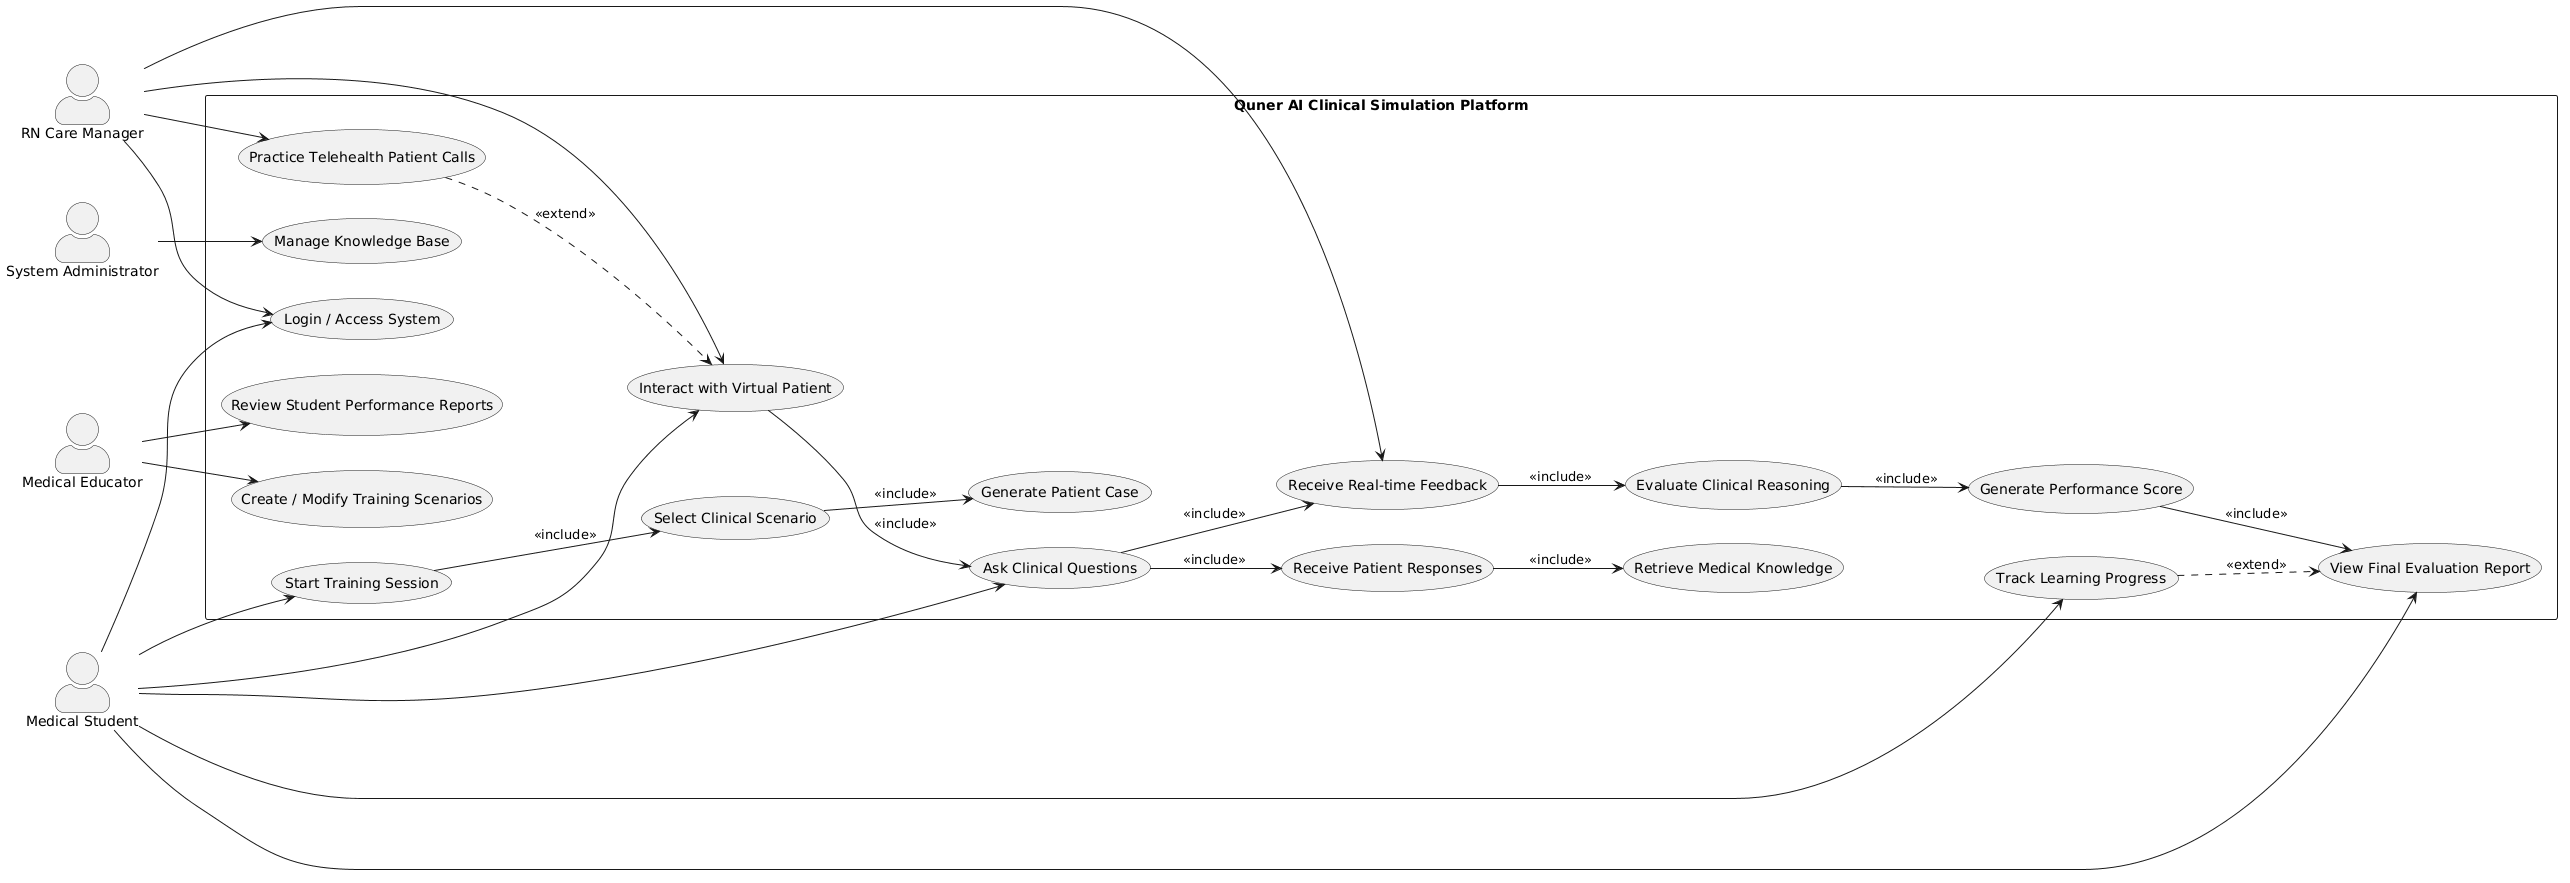
\includegraphics[angle=90, width=0.95\linewidth, keepaspectratio]{figures/quner_usecase.png}
    \caption{Use Case Diagram for the Quner training framework}
    \label{fig:quner_usecase}
\end{figure}

\subsubsection{Data Flow Diagram}
\begin{figure}[H]
    \centering
    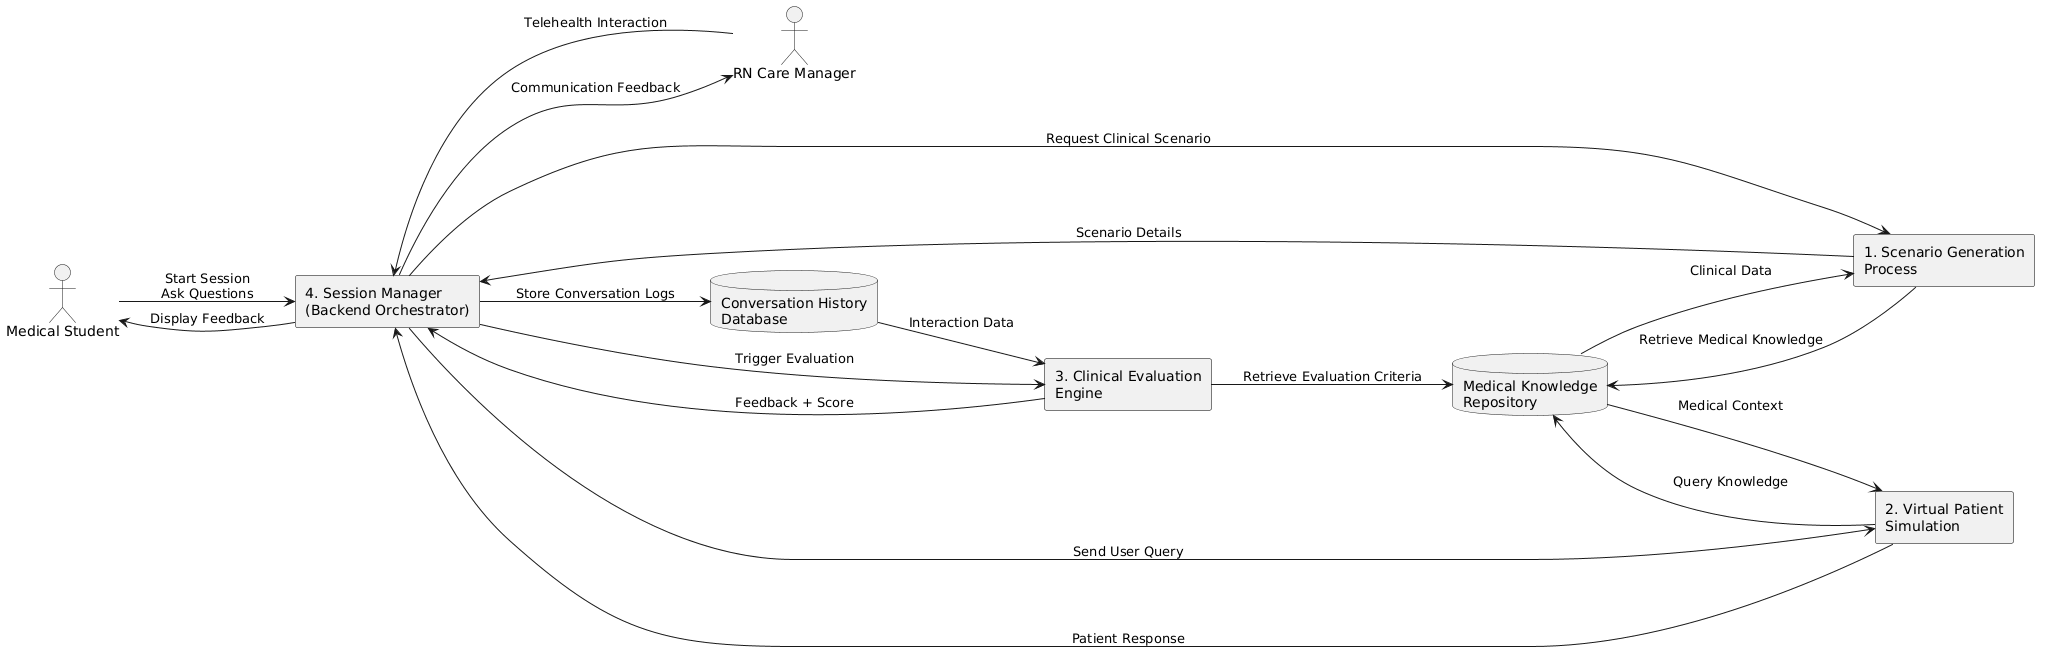
\includegraphics[angle=90, width=0.7\linewidth, keepaspectratio]{figures/quner_dataflow.png}
    \caption{Data Flow Diagram}
    \label{fig:quner_dataflow}
\end{figure}

\subsubsection{Class Diagram}
\begin{figure}[H]
    \centering
    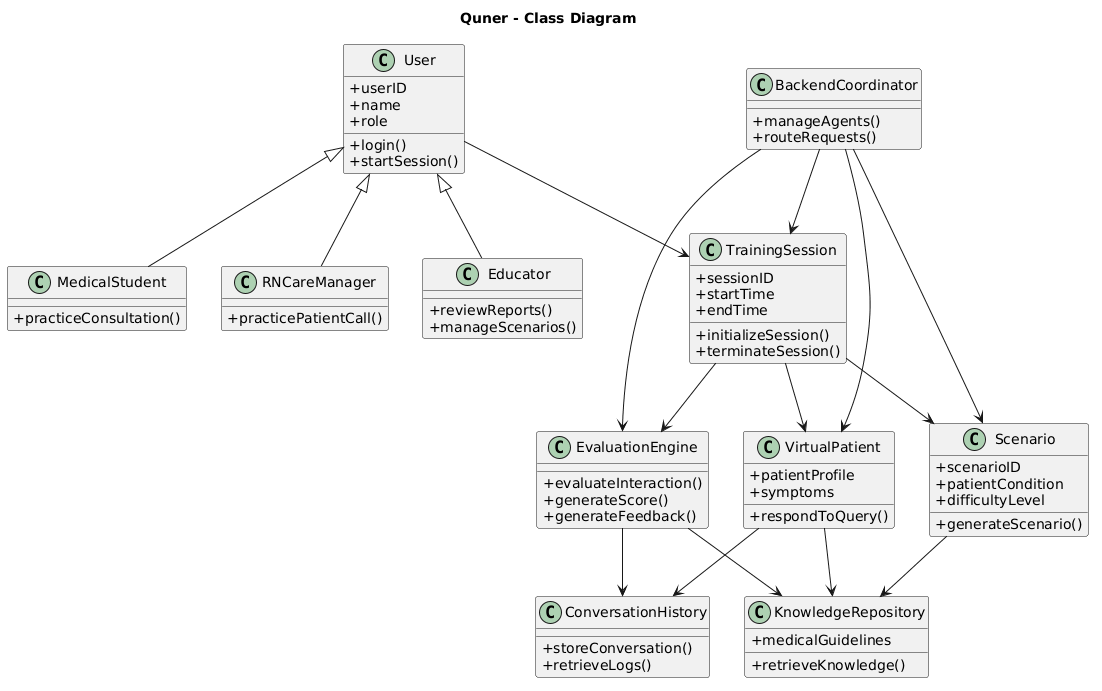
\includegraphics[width=0.9\linewidth, keepaspectratio]{figures/quner_class.png}
    \caption{Class Diagram}
    \label{fig:quner_class}
\end{figure}

\subsubsection{Sequence Diagram}
\begin{figure}[H]
    \centering
    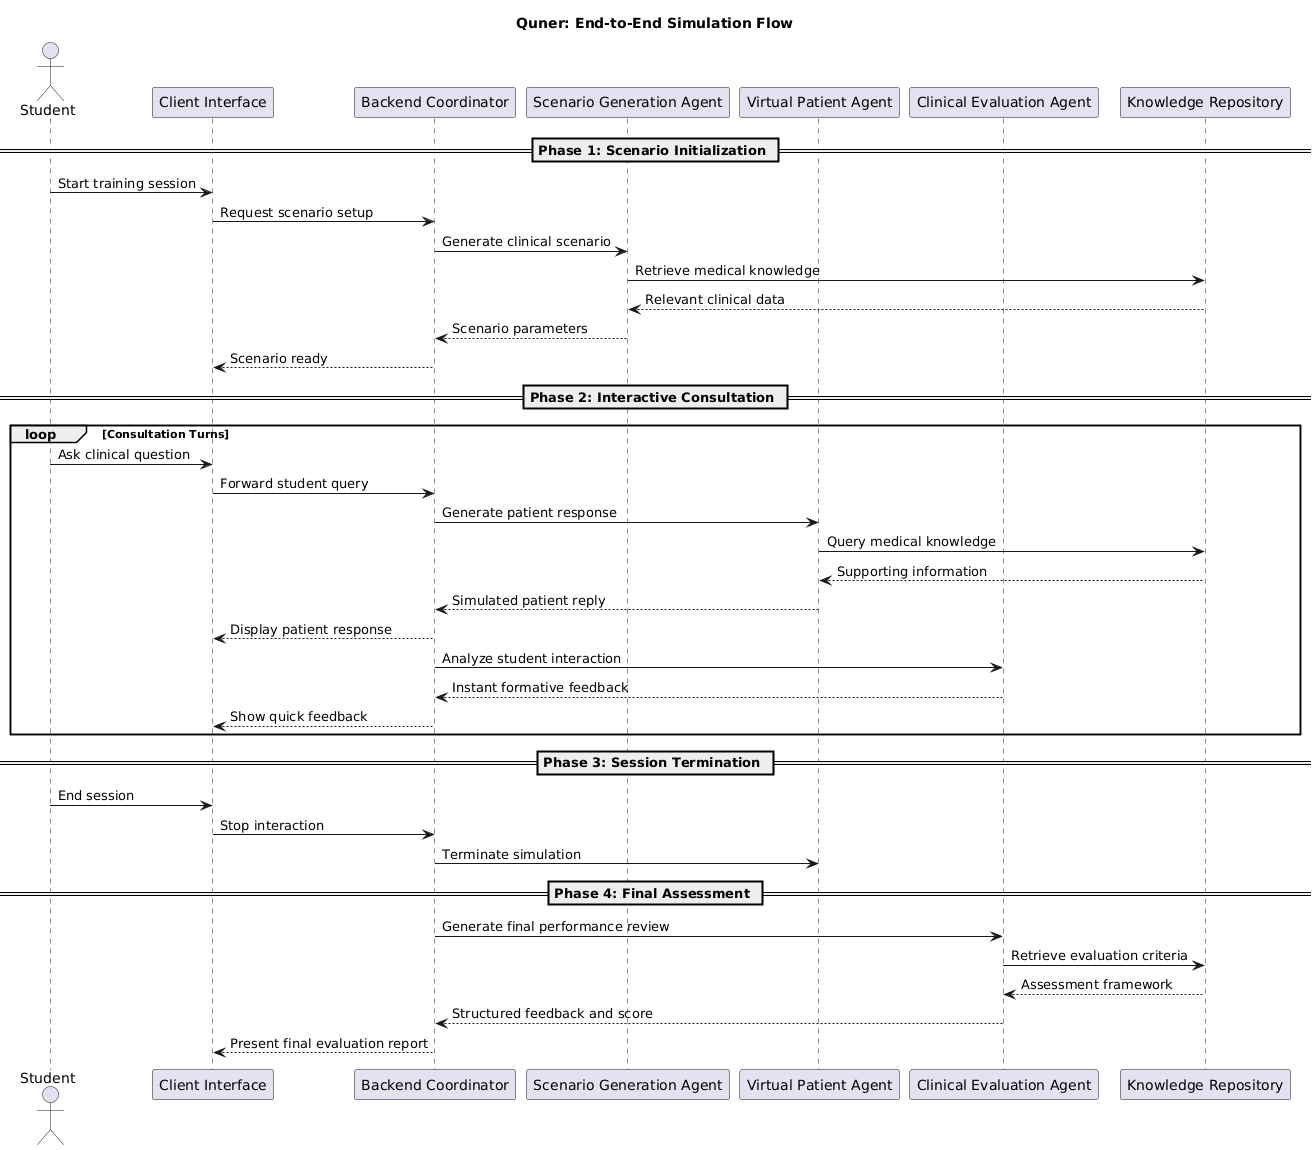
\includegraphics[width=0.9\linewidth, keepaspectratio]{figures/quner_sequenece_diagaram.png}
    \caption{Sequence Diagram}
    \label{fig:quner_sequence}
\end{figure}

\subsubsection{Component Diagram}
\begin{figure}[H]
    \centering
    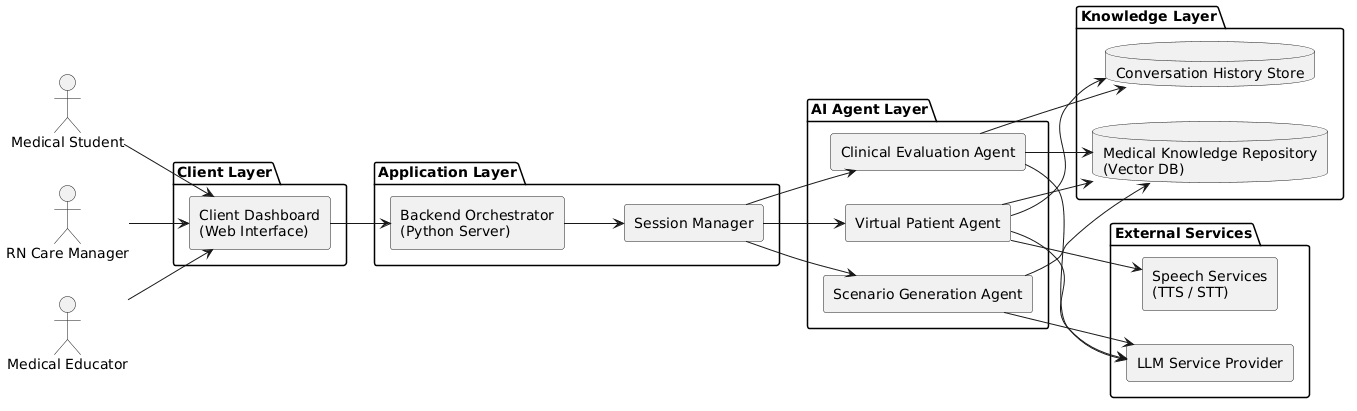
\includegraphics[width=0.9\linewidth, keepaspectratio]{figures/quner_component.png}
    \caption{Component Diagram}
    \label{fig:quner_component}
\end{figure}

\subsubsection{Architecture Diagram}
\begin{figure}[H]
    \centering
    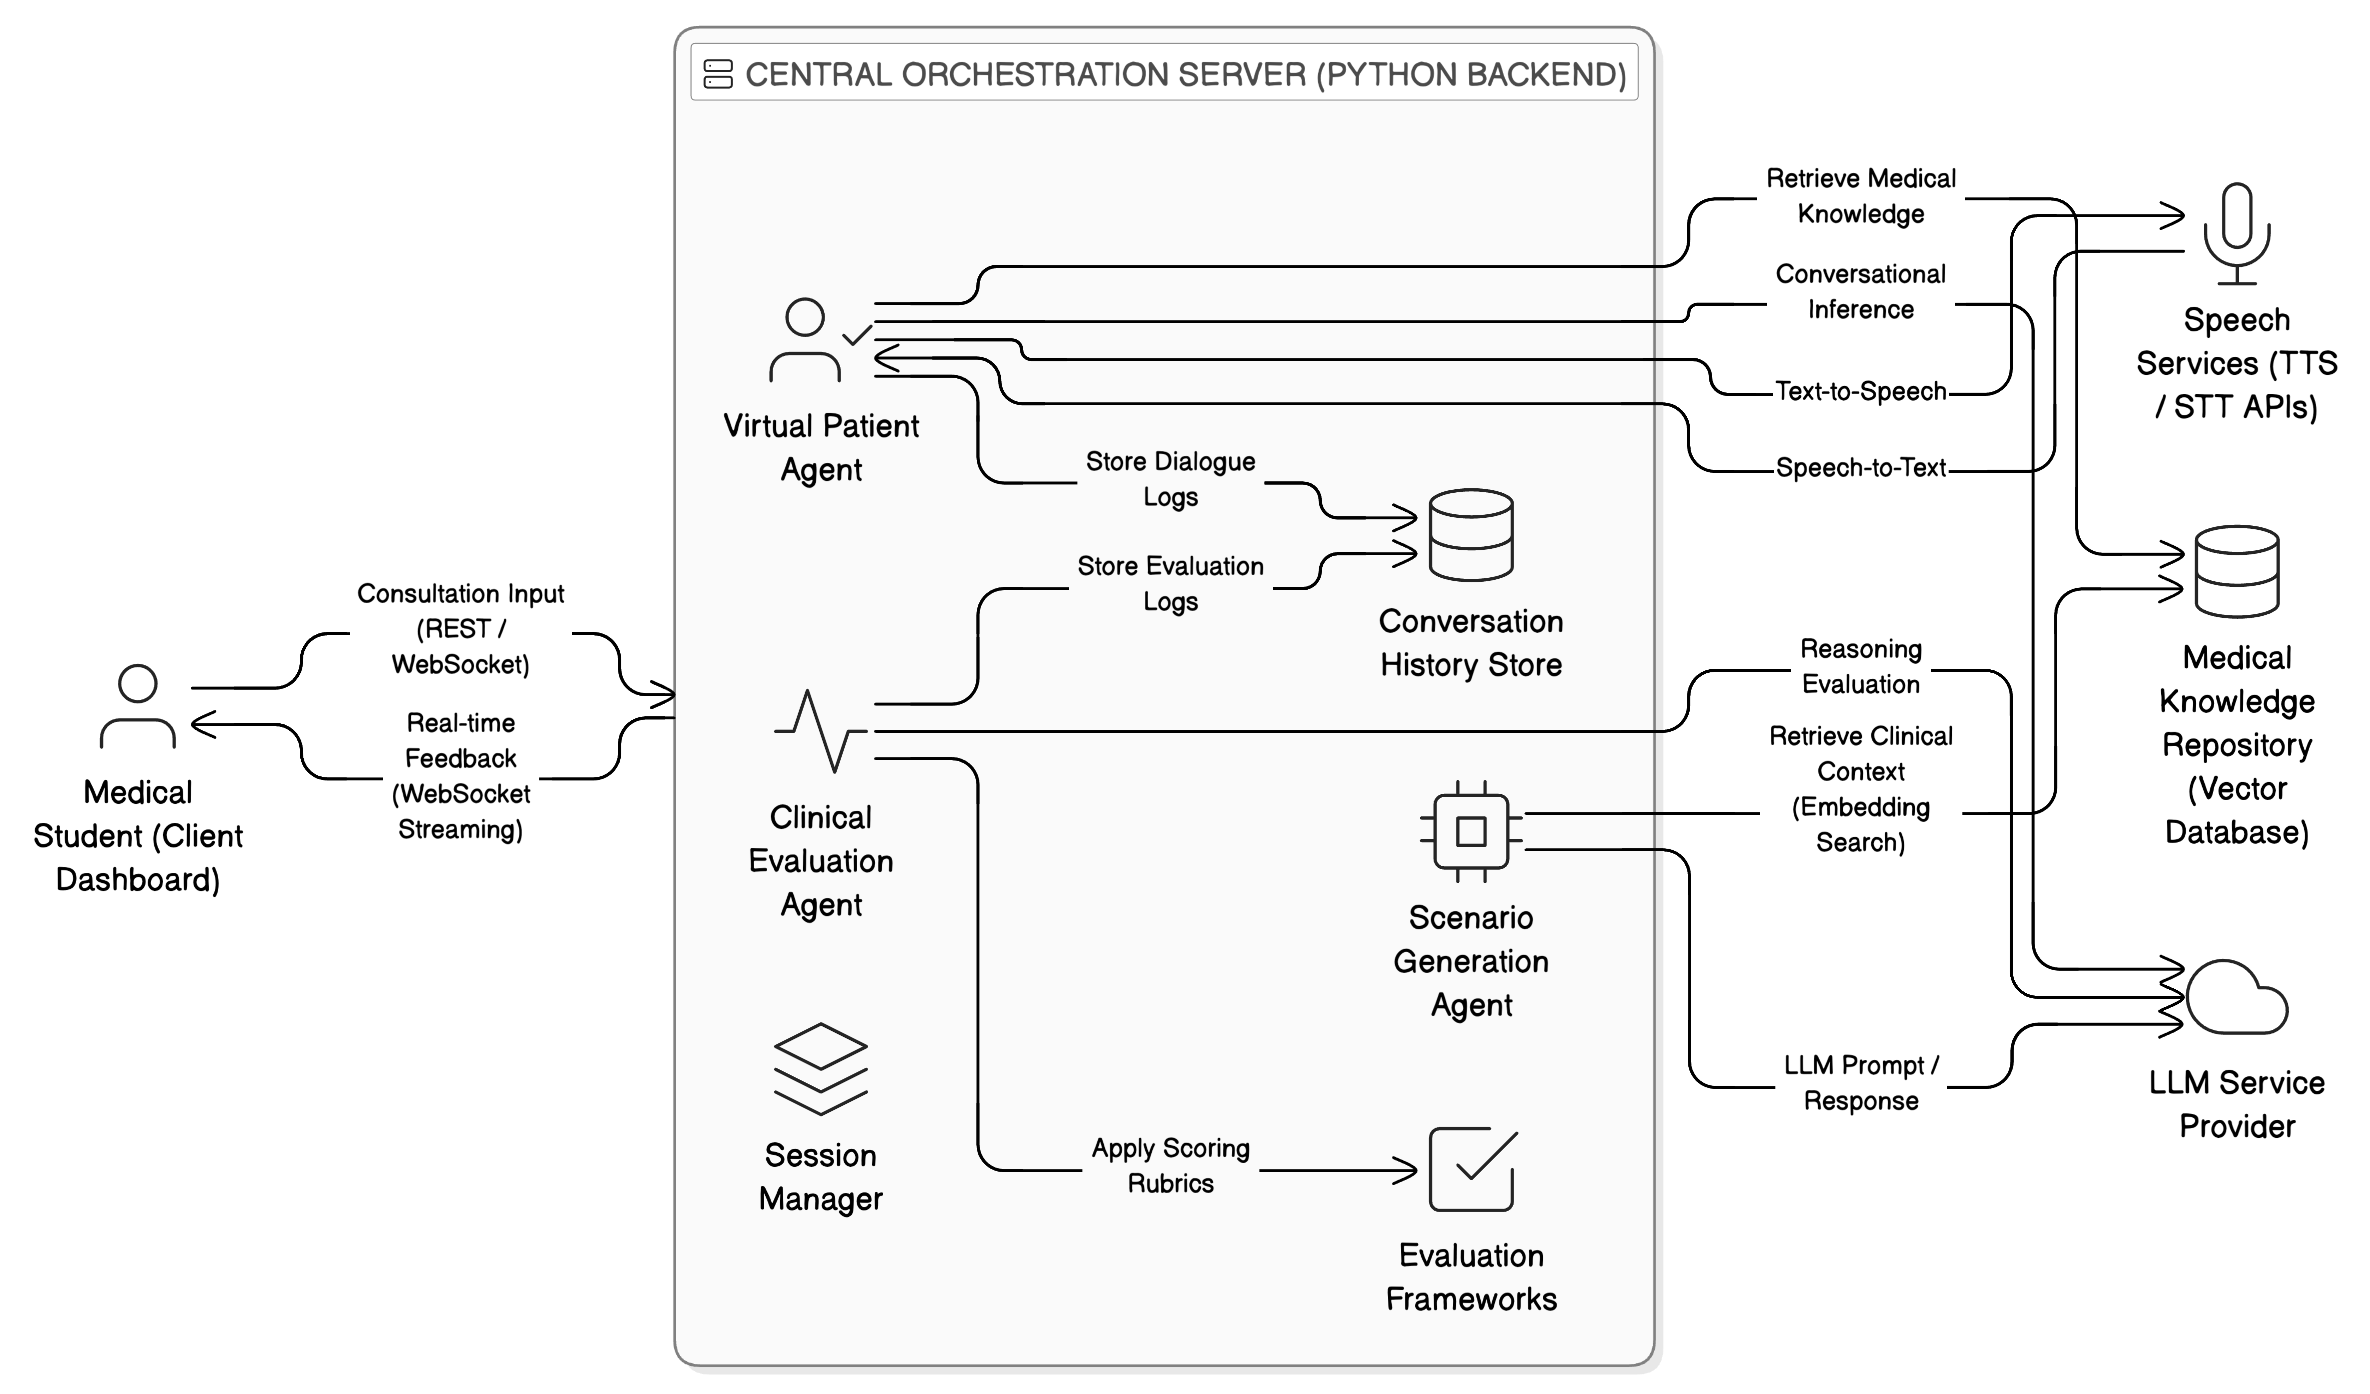
\includegraphics[angle=90, width=0.9\linewidth, keepaspectratio]{figures/quner_architecture.png}
    \caption{High-Level Architecture Diagram}
    \label{fig:quner_architecture}
\end{figure}

\subsection{SWOT Analysis}
\begin{table}[H]
\centering
\renewcommand{\arraystretch}{1.3}
\caption{SWOT Analysis of Quner}
\vspace{2mm}
\begin{tabular}{|p{7cm}|p{7cm}|}
\hline
\textbf{\vspace{1mm}Strengths\vspace{1mm}} & \textbf{\vspace{1mm}Weaknesses\vspace{1mm}} \\ \hline
\textbf{Multi-Agent Decoupling:} Generator, VSP, and Critic are independently tunable. \newline
\textbf{Pluggable LLM Backends:} OpenAI / Groq / full mode, switchable via one env var. \newline
\textbf{Structured, Transcript-Linked Feedback:} Per-criterion MIRS + 7-criterion clinical evaluation. \newline
\textbf{Browser-Native Multimodal:} STT and TTS via the Web Speech API, no extra services. \newline
\textbf{Reproducible Cases:} Every vignette persists to \texttt{generated\_patients/}.
&
\textbf{LLM Hallucination Risk:} Without RAG enabled, factual grounding depends on the model alone. \newline
\textbf{API Latency Sensitivity:} Real-time chat is bounded by provider latency. \newline
\textbf{No Physical Examination:} The system simulates dialogue, not tactile clinical exams. \newline
\textbf{Browser Compatibility:} STT requires Chromium / Safari; Firefox falls back to typing.
\\ \hline

\textbf{\vspace{1mm}Opportunities\vspace{1mm}} & \textbf{\vspace{1mm}Threats\vspace{1mm}} \\ \hline
\textbf{Rising Demand for Scalable Training:} Medical-school enrolment outpaces SP supply. \newline
\textbf{Generalisable Architecture:} The same design fits legal, customer-support, and therapy training. \newline
\textbf{LMS Integration:} MIRS / clinical scores can be exported into Moodle, Canvas, or Blackboard. \newline
\textbf{Educator Test-Bank Construction:} Persisted vignettes form a reusable test-item library.
&
\textbf{LLM Pricing Volatility:} Provider costs and rate limits change frequently. \newline
\textbf{Educator Adoption Friction:} Some faculty distrust AI-generated grading. \newline
\textbf{Regulatory Scrutiny:} Healthcare-adjacent software may attract privacy / accuracy review. \newline
\textbf{Vendor Lock-In Pressure:} Pluggable backends mitigate but do not eliminate this risk.
\\ \hline
\end{tabular}
\end{table}
\newpage

\subsection{Methodology (Agile Model -- Iterative Refactor)}

The development of Quner followed an \textbf{Agile, iteration-driven methodology} closely aligned with Extreme Programming (XP) principles \cite{Portovaras2024CurrentTA}. Because the project began with a research prototype and evolved through a series of incremental enhancements (multimodal I/O, pipeline-mode switching, modular package refactor, viewport-locked layout), an iterative process with short feedback cycles was the natural fit \cite{Topsakal2023CreatingLL}.

\subsubsection{Requirement Analysis}
Requirements were captured as \emph{user stories} from the perspective of three stakeholder groups -- educators, students, and operators -- and refined collaboratively after each demo cycle \cite{Azzara2023PeranPP}.

\begin{itemize}
    \item \textbf{User Stories (Functional):}
    \begin{itemize}
        \item As a \emph{student}, I want to type or speak to a virtual patient so I can practise interviewing without a human SP.
        \item As a \emph{student}, I want a one-line hint mid-conversation that doesn't reveal the diagnosis, so I can self-coach \cite{Krugmann2024SentimentAI}.
        \item As an \emph{educator}, I want every session to produce a structured MIRS + clinical score with transcript evidence.
        \item As an \emph{educator}, I want to replay the same vignette across a cohort for comparable assessment.
        \item As an \emph{operator}, I want to switch LLM providers without touching agent logic when costs change.
    \end{itemize}

    \item \textbf{Non-Functional:}
    \begin{itemize}
        \item Patient-reply latency target: under 5 s per turn on \texttt{gpt-4o-mini}.
        \item No hard-coded secrets, anywhere.
        \item Graceful degradation: STT failure or TTS failure must not crash the session; the chat must continue in text.
        \item Backwards compatibility: the refactor must preserve every public symbol from the original \texttt{utils.py}, \texttt{prompts.py}, \texttt{ui\_utils.py} \cite{Rygl2017SemanticVE}.
    \end{itemize}
\end{itemize}

\subsubsection{System Design}
The system was redesigned around the principle of \emph{single-responsibility modules with thin facades}.

\begin{itemize}
    \item \textbf{Backend:} Split monolithic \texttt{utils.py} into \texttt{llm/clients.py}, \texttt{llm/rag.py}, \texttt{llm/parsers.py}, \texttt{agents/generator.py}, \texttt{agents/vsp.py}, \texttt{agents/critic.py}, \texttt{agents/predefined.py}, \texttt{agents/lifecycle.py}. \texttt{utils.py} survives as a 50-line facade that re-exports the public API \cite{Cheptsov2013IntroducingAN}.

    \item \textbf{Prompts:} Split monolithic \texttt{prompts.py} into \texttt{prompts/generation.py}, \texttt{prompts/vsp.py}, \texttt{prompts/feedback.py}, \texttt{prompts/post\_processing.py}, \texttt{prompts/hint.py}, with a 90-line \texttt{prompts/\_\_init\_\_.py} that re-exports every template name.

    \item \textbf{Dashboard UI:} Split monolithic \texttt{ui\_utils.py} into \texttt{ui/state.py} (all module-level mutable state), \texttt{ui/dialogs.py}, \texttt{ui/form.py}, \texttt{ui/chat.py}, \texttt{ui/sidebar.py}, \texttt{ui/feedback\_view.py}, \texttt{ui/notifications.py}. A 60-line \texttt{ui\_utils.py} facade preserves backwards compatibility.

    \item \textbf{Configuration Surface:} Every secret and pipeline-shaping flag is read from \texttt{.env}; \texttt{config.py} is the single source of truth for what those flags mean \cite{Shen2019ALA}.

    \item \textbf{Workflow Example:} See the "Typical Simulation Flow" enumeration above for the trigger-to-feedback chain.
\end{itemize}

\subsubsection{Implementation}
Implementation followed XP practices: small commits, immediate live testing in the browser, refactor-as-you-go \cite{Stokes2015ScalingNA}.

\begin{itemize}
    \item \textbf{Agent Modules:} Generator pipeline (8 steps); VSP pre-processing $\rightarrow$ case routing $\rightarrow$ post-processing; Critic quick + final + hint.
    \item \textbf{LLM Integration:} \texttt{model\_for(stage)} dispatcher; \texttt{structured\_response\_format(schema)} that returns \texttt{json\_schema} for OpenAI and \texttt{json\_object} for Groq.
    \item \textbf{Browser JavaScript Bridge:} \texttt{coworkSpeak()}, \texttt{coworkToggleMic()}, \texttt{coworkSetAutoSubmit()}, plus a wrapper-div trick to find the real \texttt{<input>} inside Quasar's \texttt{q-input} for STT injection.
    \item \textbf{XP Practices:} Iterative live demos; immediate refactor-on-discovery; user-driven scope adjustments (e.g., the voice-picker dropdown was added, then removed at the user's request).
\end{itemize}

\subsubsection{Testing \& Evaluation}
Testing combined deterministic compile / import checks with live behavioural runs.

\begin{itemize}
    \item \textbf{Static Checks:} Every change ran through \texttt{python -m py\_compile} on the affected files.
    \item \textbf{Import-Chain Smoke Test:} A scripted import of \texttt{utils} (with stubbed \texttt{openai} / \texttt{mdextractor}) confirmed every public function survives the refactor.
    \item \textbf{Live Conversations:} Generated and predefined patients were exercised end-to-end through the dashboard.
    \item \textbf{Edge Cases:} Mic toggled mid-recognition (auto-submit suppressed); TTS toggled off mid-utterance (\texttt{speechSynthesis.cancel()} fires); rate-limit responses from Groq surfaced as visible error notifications.
\end{itemize}

\subsubsection{Deployment \& Scalability}
\begin{itemize}
    \item Two independent processes, both reading the same \texttt{.env}.
    \item Tested locally on macOS (Apple Silicon) with Python 3.13 and NiceGUI 1.4.x.
    \item The two processes are designed for separate Dockerisation and can be hosted on any Linux instance with outbound HTTPS to the chosen LLM provider.
\end{itemize}

\newpage
\subsubsection{Project Plan}

The following Gantt chart represents the actual progression of Quner across the Major Project II window.\\[2ex]

\begin{center}
\begin{ganttchart}[vgrid, hgrid]{1}{15}
\gantttitle{Quner Project Plan (Major II)}{15} \\
\gantttitlelist{1,...,15}{1} \\

\ganttgroup{Phase 1: Audit \& Hardening}{1}{3} \\
\ganttbar{Codebase audit, .env migration}{1}{1} \\
\ganttlinkedbar{Pipeline-mode dispatcher (OpenAI / Groq / full)}{2}{2} \\
\ganttlinkedbar{Optional RAG bootstrap}{3}{3} \ganttnewline

\ganttgroup{Phase 2: Multimodal UI}{4}{7} \\
\ganttbar{Browser text chat (Furhat-optional path)}{4}{4} \\
\ganttlinkedbar{Web Speech API STT \& TTS}{5}{5} \\
\ganttlinkedbar{Auto-submit, hint button}{6}{6} \\
\ganttlinkedbar{Right-slide vignette drawer}{7}{7} \ganttnewline

\ganttgroup{Phase 3: Modular Refactor}{8}{11} \\
\ganttbar{Split prompts.py into prompts/ package}{8}{8} \\
\ganttlinkedbar{Split utils.py into llm/ + agents/}{9}{10} \\
\ganttlinkedbar{Split ui\_utils.py into ui/ package}{11}{11} \ganttnewline

\ganttgroup{Phase 4: UX Polish \& Validation}{12}{15} \\
\ganttbar{Viewport-locked single-screen layout}{12}{12} \\
\ganttlinkedbar{Restart-with-same-settings}{13}{13} \\
\ganttlinkedbar{End-to-end smoke testing}{14}{14} \\
\ganttlinkedbar{Final report \& documentation}{15}{15} \\
\ganttmilestone{Final Presentation}{15}

\end{ganttchart}
\end{center}

\newpage
% ----------------------------------------------------------------------------
% Implementation
% ----------------------------------------------------------------------------
\section{Implementation}

\subsection{Project Structure}

\subsubsection{Root Level Project Overview}

Quner is a two-process Python application: a backend WebSocket hub (\texttt{ws\_server.py}) that orchestrates three cooperating agents, and a NiceGUI browser dashboard (\texttt{main.py}) that connects to the hub as a "dashboard" client. The two processes share the same project-root \texttt{.env} and are otherwise independent \cite{Cheptsov2013IntroducingAN}.

The repository is organised so that each concern has its own focused package. The original prototype shipped one 844-line \texttt{utils.py}, one 879-line \texttt{prompts.py}, and one 653-line \texttt{ui\_utils.py}. After the Major II refactor every source file is under 250 lines and grouped by purpose (LLM, agents, prompts, UI components, state) \cite{Rygl2017SemanticVE}.

\paragraph{Frontend (NiceGUI Browser Dashboard)}
The dashboard is the primary student-facing surface. It is a NiceGUI application served on port \texttt{8501} that opens a sticky dark header, a viewport-locked split layout (chat + feedback on the left, scenario settings + view-vignette on the right), and a slide-out vignette drawer. A small embedded JavaScript module wires the Web Speech API for STT and TTS \cite{Portovaras2024CurrentTA}.

\paragraph{Backend (Python + Asyncio + LLM Providers)}
The backend hosts the agents and the WebSocket gateway. It uses \texttt{asyncio} for concurrency, the \texttt{openai} Python SDK as a single OpenAI-compatible client (pointed at OpenAI, Groq, or Cerebras depending on mode), and \texttt{websockets} for the gateway. Optional dependencies (Pinecone, LlamaIndex, HuggingFace embeddings) are imported lazily \cite{Topsakal2023CreatingLL,Monir2024VectorSearchED}.

\newpage
\subsubsection{Detailed Directory Description}

\begin{verbatim}
quner/
|-- .env                         # Secrets + pipeline flags (gitignored)
|-- .env.example                 # Template
|-- README.md                    # Quick-start + architecture overview
|-- create_rag_storage.py        # Optional: build the Pinecone EBM index
|-- central_backend_server/      # Backend (port 8085)
|   |-- ws_server.py             # Asyncio WebSocket gateway (orchestrator)
|   |-- config.py                # .env-driven configuration
|   |-- conversion_tables.py     # Disease library, Big-Five, faces, voices
|   |-- predefined_patients.py   # Eleanor, Cassian, Marcus
|   |-- globals_server.py        # Connection registry + broadcast helper
|   |-- globals_conversation_logic.py  # Patient + conversation state
|   |-- utils.py                 # Backwards-compat facade (50 lines)
|   |-- prompts/                 # ALL prompt templates
|   |   |-- __init__.py          #   re-exports the flat namespace
|   |   |-- generation.py
|   |   |-- vsp.py
|   |   |-- feedback.py
|   |   |-- post_processing.py
|   |   `-- hint.py
|   |-- llm/                     # Client setup + RAG + parsers
|   |   |-- __init__.py
|   |   |-- clients.py           #   OpenAI / Groq / Cerebras + model_for
|   |   |-- rag.py               #   Lazy Pinecone + LlamaIndex
|   |   `-- parsers.py           #   markdown + face/voice JSON helpers
|   |-- agents/                  # The three agents + glue
|   |   |-- __init__.py
|   |   |-- generator.py         #   8-step vignette pipeline
|   |   |-- vsp.py               #   Routing + post-processing dialogue
|   |   |-- critic.py            #   Quick + final feedback + hint
|   |   |-- predefined.py        #   Hard-coded patient launcher
|   |   `-- lifecycle.py         #   stop_patient + save_patient_artifact
|   |-- minimal_generate_client.py  # CLI test harness for Generator only
|   `-- generated_patients/      # Persisted vignettes (auto-created)
`-- client_dashboard/            # Dashboard (port 8501)
    |-- main.py                  # NiceGUI entry point + injected JS
    |-- config.py                # WebSocket URL + retry delay
    |-- utils.py                 # WS consumer + senders
    |-- ui_utils.py              # Backwards-compat facade (60 lines)
    `-- ui/                      # UI components
        |-- __init__.py
        |-- state.py             #   All module-level mutable state
        |-- dialogs.py           #   Lazy modal dialogs
        |-- form.py              #   Sliders + Restart button
        |-- chat.py              #   chat_input + messages
        |-- sidebar.py           #   Controls + vignette drawer
        |-- feedback_view.py     #   feedback() + per-criterion rows
        `-- notifications.py     #   Progress + connection + show_hint
\end{verbatim}

\textbf{Most Important Backend Components:}
\begin{itemize}
    \item \textbf{\texttt{agents/}}: The three agents from the paper, each in its own file. Adding a new agent means dropping a file in this folder \cite{Cheptsov2013IntroducingAN}.
    \item \textbf{\texttt{llm/clients.py}}: The single source of truth for LLM provider selection and model dispatch \cite{Kulkarni2023TheEO}.
    \item \textbf{\texttt{llm/rag.py}}: Lazy RAG bootstrap; never imports the heavy stack unless \texttt{USE\_RAG=1} \cite{Monir2024VectorSearchED}.
    \item \textbf{\texttt{prompts/}}: Every template grouped by agent for navigability.
    \item \textbf{\texttt{ws\_server.py}}: 230-line action dispatcher that owns the WebSocket lifecycle \cite{Rygl2017SemanticVE}.
\end{itemize}

\paragraph{Configuration (\texttt{.env})}
Three pipeline modes are supported via a single env var:
\begin{itemize}
    \item \texttt{PIPELINE\_MODE=openai-only}: every LLM call goes through OpenAI, RAG is forced off, the \texttt{client} object is the OpenAI default.
    \item \texttt{PIPELINE\_MODE=groq-only}: every LLM call goes through Groq's OpenAI-compatible endpoint; structured-output is downgraded from \texttt{json\_schema} to \texttt{json\_object}; RAG forced off.
    \item \texttt{PIPELINE\_MODE=full}: original paper pipeline -- Cerebras for VSP preprocessing, Groq for vignette + answer generation, OpenAI for post-processing and feedback. Optional RAG via \texttt{USE\_RAG=1}.
\end{itemize}

\newpage
\subsection{Code Explanation}

The following snippets are excerpted from the refactored codebase. Each block is intentionally short -- the full sources live in the indicated module.

\subsubsection{Pipeline-Mode Dispatcher (\texttt{llm/clients.py})}

\begin{lstlisting}[style=codeblock]
from openai import OpenAI
import config

print(f"Initializing language models (PIPELINE_MODE={config.PIPELINE_MODE})...")

if config.GROQ_ONLY:
    client = OpenAI(base_url="https://api.groq.com/openai/v1/",
                    api_key=config.GROQ_API_KEY)
    cerebras_client = client
    groq_client = client
elif config.OPENAI_ONLY:
    client = OpenAI(api_key=config.OPENAI_API_KEY)
    cerebras_client = client
    groq_client = client
else:
    client = OpenAI(api_key=config.OPENAI_API_KEY)
    cerebras_client = OpenAI(base_url="https://api.cerebras.ai/v1/",
                             api_key=config.CEREBRAS_API_KEY)
    groq_client = OpenAI(base_url="https://api.groq.com/openai/v1/",
                         api_key=config.GROQ_API_KEY)


def model_for(stage: str) -> str:
    if config.GROQ_ONLY:
        return config.vignette_generation_groq_model
    if config.OPENAI_ONLY:
        return {
            "vignette": config.VSP_model_openai,
            "preprocessing": config.VSP_model_openai,
            "answergeneration": config.VSP_model_openai,
            "postprocessing": config.VSP_model_postprocessing,
            "quick_feedback": config.quick_feedback_api_model,
            "full_feedback": config.full_feedback_api_model,
        }[stage]
    return {
        "vignette": config.vignette_generation_groq_model,
        "preprocessing": config.VSP_model_preprocessing,
        "answergeneration": config.VSP_model_answergeneration,
        "postprocessing": config.VSP_model_postprocessing,
        "quick_feedback": config.quick_feedback_api_model,
        "full_feedback": config.full_feedback_api_model,
    }[stage]
\end{lstlisting}

\paragraph{}
The \texttt{llm/clients.py} module is the only place in the codebase that constructs LLM clients. The three branches above correspond to the three pipeline modes; the rest of the system never inspects \texttt{PIPELINE\_MODE} directly. Switching from a paid OpenAI deployment to Groq's free tier therefore costs one \texttt{.env} line; no agent is aware of the change \cite{Kulkarni2023TheEO}.

\subsubsection{Generator Agent -- 8-Step Vignette Pipeline (\texttt{agents/generator.py})}

\begin{lstlisting}[style=codeblock]
async def generate_patient(disease_difficulty, neuroticism, extraversion,
                           openness, agreeableness, conscientiousness):
    NR_OF_STEPS = 8
    await broadcast_message({"action": "generationStart"})

    # Step 1: pick a disease
    disease_name = random.choice(list(conversion_tables.diseases.keys()))
    disease_documents, score = conversion_tables.diseases[disease_name]
    await globals_conversation_logic.add_debug_log(
        f"1. Picked the disease: {disease_name} with a difficulty of {score}/10."
    )

    # Step 2-7: difficulty reasoning -> first draft -> consistency scan
    #           -> post-process plan -> final draft -> avatar selection
    # ... (full source in agents/generator.py)

    patient = globals_conversation_logic.Patient(
        disease=disease_name, vignette=markdown_block,
        face=face, voice=voice,
        neuroticism=conversion_tables.translate_score("neuroticism", neuroticism),
        extraversion=conversion_tables.translate_score("extraversion", extraversion),
        openness=conversion_tables.translate_score("openness", openness),
        agreeableness=conversion_tables.translate_score("agreeableness", agreeableness),
        conscientiousness=conversion_tables.translate_score("conscientiousness",
                                                            conscientiousness),
    )

    await globals_conversation_logic.start_patient(patient)
    save_patient_artifact(patient, source="generated")
\end{lstlisting}

\paragraph{}
The Generator agent runs an eight-step prompt chain on the configured \emph{vignette} model. Each step appends both its prompt and its answer to the debug log (visible in the dashboard's \emph{Generation log} dialog), so the full provenance of every produced patient is auditable \cite{Mahajan2022TextualDQ}. The final patient is persisted to \texttt{generated\_patients/<timestamp>\_<disease>.md} so the same case can be re-launched across an entire cohort \cite{Zhao2023ASO}.

\subsubsection{VSP Agent -- Routing + Post-Processing (\texttt{agents/vsp.py})}

\begin{lstlisting}[style=codeblock]
async def generate_patient_response():
    patient = globals_conversation_logic.get_patient()
    history = globals_conversation_logic.get_conversation_history()

    # Bootstrap path: first turn -> patient greets the doctor
    if len(history) == 0:
        system_prompt = prompts.conversation_new_firstmessage.substitute(...)
    else:
        # Pre-processing: classify the situation 1..6
        completion = cerebras_client.chat.completions.create(
            model=model_for("preprocessing"),
            messages=[
                {"role": "system", "content": prompts.conversation_new_preprocessing},
                {"role": "user", "content": f"...history + vignette..."},
            ],
        )
        output, database_question = _parse_output_and_question(
            completion.choices[0].message.content)

        match output:
            case 1: system_prompt = prompts.conversation_new_1.substitute(...)
            case 2: system_prompt = prompts.conversation_new_2.substitute(...)
            case 3: system_prompt = prompts.conversation_new_3.substitute(...)
            case 4: system_prompt = prompts.conversation_new_4.substitute(...)
            case 5: system_prompt = prompts.conversation_new_5.substitute(...)
            case 6:
                # RAG path (only if USE_RAG=1)
                if database_question and medical_knowledge_tool:
                    rag = medical_knowledge_tool.query_engine.query(...)
                    system_prompt = prompts.conversation_new_6.substitute(
                        medical_information=rag.response, ...)

    # Generate the raw answer
    completion = groq_client.chat.completions.create(
        model=model_for("answergeneration"), messages=llm_prompt)
    response = completion.choices[0].message.content

    # Post-process: enforce persona + knowledge bounds
    response = post_process(was_doctor_utterance=True,
                            answer=response,
                            conversation_history=history,
                            patient=patient)

    await broadcast_message({"action": "patientGeneratedResponse",
                             "response": response,
                             "time": datetime.now().strftime("%H:%M")})
\end{lstlisting}

\paragraph{}
The VSP agent is the most interesting piece of agent logic in the system. Every doctor utterance after the first is run through a pre-processing classifier that picks one of six conversation cases. Case 6 is the only one that consults RAG; the others use case-specific system prompts that vary the tone and constraints. After the model produces the raw answer, a separate \texttt{post\_process()} call runs on \texttt{gpt-4o-mini} with a personality-aware filter that strips doctor-vocabulary, removes diagnostic guesses, and tightens the wording to match the patient's Big-Five profile \cite{Zhang2023SentimentAI}.

\subsubsection{Critic Agent -- Hint (\texttt{agents/critic.py})}

\begin{lstlisting}[style=codeblock]
async def generate_hint():
    patient = globals_conversation_logic.get_patient()
    if patient is None:
        await broadcast_message({"action": "hintResponse",
                                 "hint": "Start a patient first."})
        return

    history = globals_conversation_logic.get_conversation_history()
    convo = "".join(
        f"{'Doctor' if e['origin']=='doctor' else 'Patient'}: {e['message']}\n"
        for e in history
    ) or "(no exchanges yet -- the patient has just walked in)"

    prompt = prompts.hint_prompt.substitute(
        vignette=patient.vignette,
        conversation=convo,
    )
    try:
        completion = client.chat.completions.create(
            model=model_for("quick_feedback"),
            messages=[{"role": "user", "content": prompt}],
            temperature=0.4,
        )
        hint = completion.choices[0].message.content.strip()
    except Exception as e:
        hint = f"Hint unavailable right now ({type(e).__name__})."

    await broadcast_message({"action": "hintResponse", "hint": hint})
\end{lstlisting}

\paragraph{}
The hint feature lets the student request a one-sentence next-step suggestion mid-conversation. The prompt is engineered to refuse to name the diagnosis, refuse to disclose vignette content the patient hasn't volunteered, and start its suggestion with an action verb (\emph{Ask\ldots}, \emph{Explore\ldots}, \emph{Consider\ldots}). This converts the Critic from a purely retrospective grader into an in-session coach \cite{Krugmann2024SentimentAI}.

\subsubsection{Critic Agent -- Final Feedback Schemas}

\begin{lstlisting}[style=codeblock]
clinical_schema = {
    "type": "object",
    "properties": {
        "diagnosis_feedback": {"type": "string"},
        "treatment_planning_feedback": {"type": "string"},
        "follow_up_and_monitoring_feedback": {"type": "string"},
        "adherence_to_guidelines_feedback": {"type": "string"},
        "risk_assessment_feedback": {"type": "string"},
        "test_and_investigation_ordering_feedback": {"type": "string"},
        "preventive_care_feedback": {"type": "string"},
    },
    "required": [...],
    "additionalProperties": False,
}
response_format = structured_response_format(clinical_schema)

per_criterion_format = structured_response_format({
    "type": "object",
    "properties": {
        "mark": {"type": "number"},
        "explanation": {"type": "string"},
        "evidence": {"type": "array", "items": {"type": "string"}},
    },
    "required": ["mark", "explanation", "evidence"],
    "additionalProperties": False,
})
\end{lstlisting}

\paragraph{}
The clinical schema produces a single JSON object covering seven evaluation criteria; the per-criterion schema runs once for every entry in \texttt{prompts.final\_feedback\_criteria} (the MIRS criteria list). On OpenAI both schemas are enforced through strict \texttt{json\_schema}; on Groq they degrade to \texttt{json\_object} mode plus prompt-side schema instructions, since Groq doesn't support the strict mode \cite{Mahajan2022TextualDQ}.

\subsubsection{Browser Speech Bridge (\texttt{client\_dashboard/main.py})}

\begin{lstlisting}[style=codeblock]
window.coworkSpeak = function(text) {
    if (!window.coworkTtsEnabled || !window.speechSynthesis) return;
    try {
        window.speechSynthesis.cancel();
        const utter = new SpeechSynthesisUtterance(text);
        utter.rate = 1.0; utter.pitch = 1.0;
        window.speechSynthesis.speak(utter);
    } catch (e) { console.warn('TTS failed:', e); }
};

function buildRecognition() {
    const SR = window.SpeechRecognition || window.webkitSpeechRecognition;
    if (!SR) { alert("Browser does not support speech recognition."); return null; }
    const r = new SR();
    r.continuous = false;        // push-to-talk
    r.interimResults = true;
    r.lang = 'en-US';
    let finalTranscript = '';
    r.onresult = (e) => {
        let interim = '';
        for (let i = e.resultIndex; i < e.results.length; i++) {
            if (e.results[i].isFinal) finalTranscript += e.results[i][0].transcript + ' ';
            else interim += e.results[i][0].transcript;
        }
        setInputValue((finalTranscript + interim).trim());
    };
    r.onend = () => {
        // Auto-submit if enabled and not user-aborted
        if (window.coworkAutoSubmit && !userManuallyStopped && hasText()) {
            setTimeout(clickSend, 150);
        }
    };
    return r;
}
\end{lstlisting}

\paragraph{}
The browser speech bridge runs entirely client-side. \texttt{coworkSpeak()} is gated on the "Speak responses" toggle and uses the system default voice. The recognition object is configured for push-to-talk (\texttt{continuous=false}); when it ends naturally and the auto-submit switch is on, a synthetic click on the Send button posts the recognized text to the backend \cite{Beloki2017ASA,Stokes2015ScalingNA}.

\subsubsection{Dashboard WebSocket Consumer (\texttt{client\_dashboard/utils.py})}

\begin{lstlisting}[style=codeblock]
async def consumer():
    global _websocket
    while True:
        try:
            async with aiohttp.ClientSession(trust_env=True) as session:
                async with session.ws_connect(config.WS_CONN) as websocket:
                    _websocket = websocket
                    await websocket.send_str('{"action":"setRole","role":"dashboard"}')
                    # Replay current state to repopulate UI on reconnect
                    for action in ("checkPatient", "getHistory", "getQuickFeedback",
                                   "recallFinalFeedback", "checkFurhatConnected",
                                   "getDebugLog", "getPatientInformation",
                                   "getConversationId"):
                        await websocket.send_str(f'{{"action":"{action}"}}')
                    async for message in websocket:
                        data = message.json()
                        # ... dispatch ~15 action types to ui_utils handlers ...
        except Exception as e:
            print(f"WS error: {e}. Retrying in {config.RETRY_DELAY}s.")
        finally:
            _websocket = None
            await asyncio.sleep(config.RETRY_DELAY)
\end{lstlisting}

\paragraph{}
The dashboard's consumer task is a single async loop that maintains the WebSocket connection. On (re)connect it replays a fixed sequence of state-query actions so the UI repopulates from the backend's current state, then listens for events and dispatches them to the right \texttt{ui\_utils} handler. Connection loss is handled by sleeping \texttt{RETRY\_DELAY} seconds and reconnecting automatically \cite{Shen2019ALA}.

\newpage
% ----------------------------------------------------------------------------
% New features added in Major II
% ----------------------------------------------------------------------------
\section{New Features Added in Major Project II}

This section enumerates the enhancements introduced during Major Project II on top of the original SRS-stage prototype. Every item below is fully implemented and is exercised in the screenshots in the next section.

\subsection{Operational Hardening}
\begin{itemize}
    \item \textbf{Externalised Secrets via \texttt{.env}.} The original \texttt{config.py} contained four API keys hard-coded as Python string literals -- a serious operational issue for any pushed commit. Major II moves all four (\texttt{OPENAI\_API\_KEY}, \texttt{GROQ\_API\_KEY}, \texttt{CEREBRAS\_API\_KEY}, \texttt{PINECONE\_API\_KEY}) plus the new pipeline-shaping flags into a project-root \texttt{.env}, loaded by \texttt{python-dotenv}. The \texttt{.env} is gitignored and a \texttt{.env.example} template is committed \cite{Shen2019ALA}.

    \item \textbf{Pipeline-Mode Dispatcher.} A single \texttt{PIPELINE\_MODE} variable selects between three modes -- \texttt{openai-only}, \texttt{groq-only}, and \texttt{full} -- and a single \texttt{model\_for(stage)} function in \texttt{llm/clients.py} owns every model name decision. Switching providers therefore costs one env-var edit and one process restart.

    \item \textbf{Optional RAG.} The Pinecone + LlamaIndex + HuggingFace embedding stack is imported lazily inside \texttt{llm/rag.py} and only when \texttt{USE\_RAG=1}. The OpenAI-only path therefore boots in well under a second and never touches the heavy dependencies \cite{Monir2024VectorSearchED}.

    \item \textbf{Furhat-Optional Architecture.} \texttt{globals\_conversation\_logic.start\_patient()} no longer treats "no Furhat" as a warning; it always broadcasts \texttt{startPatient}, allowing the dashboard to switch into chat mode regardless of robot presence. The same backend can still drive a real Furhat if one connects with \texttt{role=furhat}.
\end{itemize}

\subsection{Multimodal User Interface}
\begin{itemize}
    \item \textbf{Browser Text Chat.} A NiceGUI input + Send button row replaces the original Furhat-only voice loop. The dashboard auto-bootstraps the patient's first turn by sending \texttt{getPatientResponse} as soon as \texttt{startPatient} arrives, so the conversation kicks off with a patient greeting instead of silence \cite{Portovaras2024CurrentTA}.

    \item \textbf{Push-to-Talk Speech-to-Text.} A microphone button next to Send toggles \texttt{webkitSpeechRecognition} (or \texttt{SpeechRecognition} where available). Interim and final transcripts stream into the chat input as the user speaks; an alert is raised if the browser doesn't support the API \cite{Beloki2017ASA}.

    \item \textbf{Auto-Submit After Speaking.} A toggle that, when on, programmatically clicks the Send button when speech recognition ends. Manual mic aborts (clicking the mic again) are tracked separately so they never trigger an auto-send \cite{Stokes2015ScalingNA}.

    \item \textbf{Text-to-Speech for Patient Replies.} A "Speak responses" switch routes every \texttt{patientGeneratedResponse} through the browser's \texttt{SpeechSynthesis} API with the system default voice. The toggle gates a single \texttt{coworkSpeak()} JavaScript function called from \texttt{add\_patient\_message()}.

    \item \textbf{Hint Button (Mid-Session Coaching).} A lightbulb button next to Send sends a \texttt{getHint} action; the Critic agent replies with a one-sentence next-step suggestion that is forbidden from naming the diagnosis. The hint pops up as a top notification with a dismiss button \cite{Krugmann2024SentimentAI}.

    \item \textbf{Right-Slide Vignette Drawer.} A \texttt{ui.dialog().props("position=right")} 480-px-wide panel that holds the full vignette in a scrollable area, opened on demand from a "View patient vignette" button. The drawer replaces the previous modal-button experience and lets the student keep the case in view during the chat.

    \item \textbf{Restart with Same Settings.} The most recent launch is tracked (\emph{generated} or \emph{predefined N}); a Restart button re-runs the same generation parameters or relaunches the same predefined patient with one click.

    \item \textbf{Viewport-Locked Single-Screen Layout.} The page itself never scrolls; only the chat area does. The header is fixed; the conversation flexes to fill the available height; the immediate-feedback card is capped at 130 px with internal scroll. The right column has its own internal scroll for narrow viewports.

    \item \textbf{Polished Theme.} Sticky dark header with the project name and avatar status; emerald-green primary actions; Tailwind-style spacing; custom scrollbars; mic-active red-pulse styling.
\end{itemize}

\subsection{Backend Capability}
\begin{itemize}
    \item \textbf{Hint Backend Path.} \texttt{generate\_hint()} in \texttt{agents/critic.py} plus a \texttt{getHint} action handler in \texttt{ws\_server.py} (with a graceful "no patient yet" path).

    \item \textbf{Full Vignette over WebSocket.} \texttt{patientInformation} now carries a \texttt{fullVignette} field so the side-drawer can render the complete vignette without an extra round-trip.

    \item \textbf{Synthetic Doctor Bootstrap.} The VSP agent injects a \emph{[Doctor enters the room and is ready to begin.]} synthetic user turn for the first patient utterance, since OpenAI rejects system-only prompts.

    \item \textbf{EBM-Optional Final Feedback.} \texttt{final\_feedback()} now tolerates missing EBM documents and falls back to "use general medical knowledge" instead of crashing on a \texttt{FileNotFoundError}.

    \item \textbf{JSON-Object Fallback for Groq.} \texttt{structured\_response\_format()} returns \texttt{json\_schema} for OpenAI but \texttt{json\_object} for Groq (which doesn't support strict schemas), and the prompts append a schema-shape instruction in Groq mode so the output stays parseable \cite{Mahajan2022TextualDQ}.
\end{itemize}

\subsection{Codebase Quality}
\begin{itemize}
    \item \textbf{Modular Refactor of Backend.} The 844-line \texttt{utils.py} is now a 50-line facade re-exporting from \texttt{llm/clients.py}, \texttt{llm/rag.py}, \texttt{llm/parsers.py}, and the five files in \texttt{agents/}. Each split file is single-responsibility \cite{Cheptsov2013IntroducingAN}.

    \item \textbf{Modular Refactor of Prompts.} The 879-line \texttt{prompts.py} is now a \texttt{prompts/} package (5 submodules + an \texttt{\_\_init\_\_.py} facade), grouped by agent.

    \item \textbf{Modular Refactor of Dashboard UI.} The 653-line \texttt{ui\_utils.py} is now a 60-line facade over a \texttt{ui/} package with seven focused submodules (state, dialogs, form, chat, sidebar, feedback\_view, notifications).

    \item \textbf{NiceGUI 2.x Compatibility Layer.} Lazy dialog creation (\texttt{fresh\_*\_dialog()} now creates the underlying \texttt{ui.dialog()} only the first time it runs) plus pinning to \texttt{nicegui<2.0} so the dashboard works against either generation of the framework \cite{Rygl2017SemanticVE}.

    \item \textbf{Backwards-Compatible Facades.} Every public symbol from the original \texttt{utils.py}, \texttt{prompts.py}, and \texttt{ui\_utils.py} is preserved through facade modules, so legacy call sites continue to work without modification.
\end{itemize}

\newpage
% ----------------------------------------------------------------------------
% Results and output (screenshots placeholders)
% ----------------------------------------------------------------------------
\section{Results and Output}

The following figures demonstrate Quner running end-to-end. All screenshots come from a live browser session against the OpenAI-only deployment with a freshly generated patient.

\subsection{Dashboard Overview}

\begin{figure}[H]
    \centering
    \screenshotplaceholder{dashboard\_overview.png}{Quner dashboard immediately after page load: sticky header, scenario settings, empty conversation log.}
    \caption{Dashboard overview: viewport-locked single-screen layout.}
    \label{fig:dashboard_overview}
\end{figure}

Figure \ref{fig:dashboard_overview} shows the dashboard at first load, before any patient is selected. The sticky header carries the project name and the avatar status icon. The left column hosts the conversation log; the right column hosts the scenario-settings card and the \emph{View patient vignette} button.

\subsection{Patient Generation in Progress}

\begin{figure}[H]
    \centering
    \screenshotplaceholder{generation\_in\_progress.png}{Top-right ongoing notification ticking through the eight-step pipeline (e.g., "Generating the first version of the patient... (3/8)").}
    \caption{Eight-step generation pipeline progress notification.}
    \label{fig:generation_progress}
\end{figure}

Figure \ref{fig:generation_progress} captures the Generator agent in mid-flight. Each \texttt{generationUpdate} event from the backend updates the on-screen progress notification with the current step number and a human-readable description.

\subsection{Live Chat with the Virtual Patient}

\begin{figure}[H]
    \centering
    \screenshotplaceholder{chat\_session.png}{Conversation log showing alternating doctor and patient bubbles, with the doctor input row + mic button + lightbulb hint button + Send below the chat scroll area.}
    \caption{Live chat session: persona-consistent dialogue with text + speech I/O.}
    \label{fig:chat_session}
\end{figure}

Figure \ref{fig:chat_session} shows a live consultation. Doctor utterances appear right-aligned with the doctor avatar; patient replies appear left-aligned with the patient avatar. The skeleton placeholder beneath the most recent doctor utterance is visible while the VSP agent generates the next reply.

\subsection{Right-Slide Vignette Drawer}

\begin{figure}[H]
    \centering
    \screenshotplaceholder{vignette\_drawer.png}{Drawer slid in from the right edge containing the full Markdown-rendered vignette with a header bar and close button.}
    \caption{Right-slide vignette drawer: full case file accessible mid-chat.}
    \label{fig:vignette_drawer}
\end{figure}

Figure \ref{fig:vignette_drawer} shows the slide-out vignette drawer overlaying the right side of the chat. Clicking the \emph{View patient vignette} button slides this 480-px panel in from the right edge; closing it returns the layout to the previous viewport-locked state.

\subsection{Hint Notification}

\begin{figure}[H]
    \centering
    \screenshotplaceholder{hint\_notification.png}{Top notification with a lightbulb prefix containing the Critic agent's one-sentence suggestion (e.g., "Ask the patient about previous similar episodes and any alleviating factors.").}
    \caption{Hint notification: on-demand mid-session coaching from the Critic agent.}
    \label{fig:hint_notification}
\end{figure}

Figure \ref{fig:hint_notification} shows the hint notification produced after the student clicks the lightbulb. The Critic agent obeys its prompt-level constraints: it never names the diagnosis, never reveals undisclosed vignette content, and starts the suggestion with an action verb.

\subsection{Final Feedback Dialog}

\begin{figure}[H]
    \centering
    \screenshotplaceholder{feedback\_dialog\_communication.png}{Modal dialog with the "Feedback on conversation" tab active, showing per-MIRS-criterion rows with a colour-coded score, the criterion name, the textual explanation, and the transcript-evidence quotes.}
    \caption{Final feedback (communication tab): per-criterion MIRS scoring with transcript evidence.}
    \label{fig:feedback_communication}
\end{figure}

Figure \ref{fig:feedback_communication} shows the communication-feedback tab. Every criterion is rendered as one row with a circle-coloured score (red = 1--2, yellow = 3, green = 4--5), the criterion name, the explanation, and quoted transcript lines that justify the score.

\begin{figure}[H]
    \centering
    \screenshotplaceholder{feedback\_dialog\_clinical.png}{The same modal switched to the "Feedback on clinical ability" tab, listing the seven clinical criteria (Diagnosis, Treatment planning, Follow-up and monitoring, Adherence to guidelines, Risk assessment, Test ordering, Preventive care) with their respective feedback paragraphs.}
    \caption{Final feedback (clinical tab): seven-criterion structured clinical evaluation.}
    \label{fig:feedback_clinical}
\end{figure}

Figure \ref{fig:feedback_clinical} shows the clinical-feedback tab of the same modal. The seven criteria are produced as a single LLM call with a strict JSON schema (or json\_object plus prompt-side instructions on Groq).

\subsection{Generation Log Dialog}

\begin{figure}[H]
    \centering
    \screenshotplaceholder{generation\_log.png}{Modal dialog scrolled to step 6 of the generation pipeline showing the prompt that was sent to the model and the markdown-formatted vignette that came back.}
    \caption{Generation log: full prompt + answer trail for the eight-step Generator pipeline.}
    \label{fig:generation_log}
\end{figure}

Figure \ref{fig:generation_log} shows the generation-log dialog. Every prompt and every answer in the eight-step Generator pipeline is appended to the log; educators can audit the full chain from disease pick to face/voice selection to confirm that the produced vignette matches their intended difficulty.

\subsection{Persisted Patient Artifact}

\begin{figure}[H]
    \centering
    \screenshotplaceholder{generated\_patient\_md.png}{File browser or text-editor screenshot showing a generated\_patients/<timestamp>\_<disease>.md file with the metadata table at the top followed by the full vignette body.}
    \caption{Persisted patient artifact: every generated case is saved as a Markdown file for cohort replay.}
    \label{fig:generated_patient_md}
\end{figure}

Figure \ref{fig:generated_patient_md} shows the on-disk artifact written by \texttt{save\_patient\_artifact()} after every successful Generator run and every predefined launch. Each file carries a metadata table (source, conversation ID, face, voice) plus the full vignette body so the same case can be re-launched across an entire cohort \cite{Mahajan2022TextualDQ}.

\newpage
% ----------------------------------------------------------------------------
% System requirements
% ----------------------------------------------------------------------------
\section{System Requirements}

The system requirements below define the hardware and software needed to run Quner in its OpenAI-only mode (the default and lightest configuration). Full-pipeline mode with RAG enabled requires additional resources for the embedding model and Pinecone index.

\subsection{Hardware Requirements (Host / Server)}

\begin{enumerate}[label=\alph*.]
    \item \textbf{Processor:} Minimum Dual-Core CPU (Intel i3 / AMD Ryzen 3 / equivalent cloud vCPU). Recommended Quad-Core for handling concurrent sessions.
    \item \textbf{Memory (RAM):} Minimum 4 GB; recommended 8 GB. The OpenAI-only path stays under 200 MB of resident memory; the RAG path adds 1--2 GB for the HuggingFace embedding model.
    \item \textbf{Storage:} 1 GB of free disk space for the application plus per-session storage for the \texttt{generated\_patients/} folder (each artifact is roughly 10--20 KB).
    \item \textbf{Network:} Stable broadband (50 Mbps minimum). All LLM calls go over outbound HTTPS to the configured providers; latency is dominated by provider response time.
\end{enumerate}

\subsection{Software Requirements}

\subsubsection{Operating System (Host)}
\begin{enumerate}[label=\alph*.]
    \item Linux (Ubuntu 20.04 LTS or later, Debian 11+, or any modern Linux distribution).
    \item macOS 11 (Big Sur) or later (Apple Silicon or Intel).
    \item Windows 10 / 11 (WSL2 strongly recommended for the dashboard).
\end{enumerate}

\subsubsection{Runtime \& Dependencies}
\begin{enumerate}[label=\alph*.]
    \item \textbf{Language Runtime:} Python 3.10 or higher (tested on 3.10 and 3.13).
    \item \textbf{Package Manager:} \texttt{pip}.
    \item \textbf{Core Python Packages (minimal install):} \texttt{openai}, \texttt{mdextractor}, \texttt{websockets}, \texttt{python-dotenv}, \texttt{nicegui<2.0}, \texttt{aiohttp}.
    \item \textbf{Optional RAG Packages:} \texttt{llama-index}, \texttt{llama-index-embeddings-huggingface}, \texttt{llama-index-vector-stores-pinecone}, \texttt{pinecone}, \texttt{pinecone-client}.
\end{enumerate}

\subsubsection{Browser (for Dashboard Use)}
\begin{enumerate}[label=\alph*.]
    \item \textbf{Recommended:} Google Chrome, Microsoft Edge, or Safari (full STT + TTS support via the Web Speech API).
    \item \textbf{Acceptable:} Firefox -- TTS works; STT silently falls back to typing because Firefox does not ship \texttt{webkitSpeechRecognition}.
\end{enumerate}

\subsubsection{External Service Dependencies}
\begin{enumerate}[label=\alph*.]
    \item \textbf{OpenAI API key} (default deployment). Roughly \$0.02 per typical session on \texttt{gpt-4o-mini}.
    \item \textbf{Groq API key} (free tier, optional alternative). Subject to a daily token cap.
    \item \textbf{Cerebras API key} (only required for \texttt{full} pipeline mode).
    \item \textbf{Pinecone account + index} (only required for \texttt{USE\_RAG=1}).
\end{enumerate}

\newpage
% ----------------------------------------------------------------------------
% Bibliography
% ----------------------------------------------------------------------------
\nocite{*}
\bibliographystyle{IEEEtran}
\bibliography{references}

\end{document}
